%
% DSP Report Template
%
% (c) 2005 EMT DSP Group
%
\documentclass[12pt,a4paper]{article}
%\usepackage{dsp_report}

\usepackage{parskip}

% randausgleich bei kleinen zeichen mit wenig deckung rechts
% % http://latex.tugraz.at/latex/fortgeschrittene#optischer_randausgleich
\usepackage[activate=normal]{pdfcprot}

\usepackage{graphicx}
\usepackage{amstext}
\usepackage{amsmath}
\usepackage{isoent} % \sfrac
\usepackage{wasysym} % \diameter
\usepackage{units}

\usepackage{txfonts} % upright \mu => \muup $math env only$
\usepackage{eurosans} % EUR sign


\usepackage{subfigure}
\usepackage{xspace}                   % space nach makro
\usepackage[left]{eurosym}            % Euro symbol
\usepackage{needspace} %preserve some space before page break, e.g. at a listings heading
\usepackage{hyperref}

\newcommand{\mbnote}[1]{\textcolor{Gray}{\textbf{\noindent M. Brandner NOTE: #1}}}
\newcommand{\mmnote}[1]{\textcolor{Gray}{\textbf{\noindent M. Maier NOTE: #1}}}
\newcommand{\MH}{\emph{``Mostly Harmless''} RoboCup Team\xspace}
\newcommand{\MSL}{Middle Size League\xspace}
\newcommand{\robocup}{\emph{RoboCup}\xspace}
\newcommand{\EMT}{Institute of Electrical Measurement and Measurement Signal Processing}

\hyphenation{VCSEL}

\begin{document}

%% Based on a TeXnicCenter-Template by Tino Weinkauf.
%%%%%%%%%%%%%%%%%%%%%%%%%%%%%%%%%%%%%%%%%%%%%%%%%%%%%%%%%%%%%

%%%%%%%%%%%%%%%%%%%%%%%%%%%%%%%%%%%%%%%%%%%%%%%%%%%%%%%%%%%%%
%% Deckblatt
%%%%%%%%%%%%%%%%%%%%%%%%%%%%%%%%%%%%%%%%%%%%%%%%%%%%%%%%%%%%%
%%
%% ATTENTION: You need a main file to use this one here.
%%            Use the command "\input{filename}" in your
%%            main file to include this file.
%%
\begin{titlepage}

  \begin{center}
    \begin{minipage}[htb]{18cm}
      \hspace*{-2.6cm}
      
\includegraphics[width=3.3cm]{./figures/logos/LogoEMT.pdf}
      \begin{tabular}{p{10cm}}\centering{
      \Large Institute of Electrical Measurement and Measurement Signal Processing\\ Graz University of Technology
      ~\\
      ~\\}
      \end{tabular}
      
\includegraphics[width=3.3cm]{./figures/logos/TUG.pdf}
    \end{minipage}

    \Large {Bachelor's Thesis\\} %
    \vspace*{1cm} \huge{\textbf{Odometry for Wheeled Mobile Robots}\\}
    %
    \vspace*{1.0cm} 
    %\Huge{\textbf{#1}\\}\vspace*{2.5cm} \vfill
    \Large{Michael Maier\\} \vspace*{1cm}
    %
    \Large{Supervisor: Dipl.-Ing. Dr. Markus Brandner\\} \vspace*{2.5cm}%


    \begin{minipage}[htb]{18cm}
      \hspace*{-0.4cm}
      
\includegraphics[width=3cm]{./figures/logos/MH.jpg}
      \begin{tabular}{p{10cm}}\centering{
        \Large Mostly Harmless RoboCup Team \\Institute for Software Technology, \\Graz University of Technology\\
        \texttt{team@robocup.tugraz.at}\\ \texttt{http://www.robocup.tugraz.at}
        ~\\
        ~\\}
      \end{tabular}
    \end{minipage}

    \Large{Graz, \today}

  \end{center}
\end{titlepage}


\tableofcontents
\clearpage
\pagestyle{plain}


\begin{abstract}
Abstract

% 1p
\end{abstract}

\clearpage

\section{Introduction}


\subsection{RoboCup}

The RoboCup is an international research and education initiative. 
Its goal is \emph{``By the year 2050, develop a team of fully autonomous robots that can win against the current human soccer world champion team"}~\cite{robocup.org}.
It promotes research in the field of robotics, e.g.\ machine vision, machine learning and autonomous systems.\\
Every year a world championship is accompanied by a conference in a different city around the globe.
In addition, various local competitions and conferences are held by local groups.\\
The RoboCup is split into three division: RoboCup Soccer, Rescue and @Home.
Every division is divided into several leagues targeted at different challenges.

%|| to Apollo Program.
%1/2 page

\subsection{\MSL}

In RoboCup Soccer the \MSL is most challenging.
The robots have to be fully autonomous.
All sensors, actuators and computation are on board and no external input is allowed.
A team consists of maximal 6~robots with a size of max.\ $50\times50\times80$\,cm$^3$.\\
The game is played on a field of $12\times18$\,m$^2$ and lasts $2\times15$~minutes.
The game field surface is generally carpet.
The \MSL is the only league where an official FIFA ball is used.
Objects are distinguished by colour: the game field is green with white lines, robots and referees are black and the ball is red.\\
The rules are the official FIFA rules~\cite{msl-rules} with slight adaptations for robotic players.
The rules are tightened every year to keep up with the technological progress. 
For instance the field size has grown from $6\times8$\,m$^2$ to $12\times18$\,m$^2$ since the introduction of the \MSL.\\
More than 20 teams from all over the world participate in the \MSL, almost all with academic background.

% 1/2 p

\subsection{\MH}

The \MH participates in the \MSL. 
Its name is a reference to the ``Hitchhiker's Guide to the Galaxy'' by Douglas Adams~\cite{h2g2}.
It was founded at Graz University of Technology at the Institute for Software Technology in 2003. 
This RoboCup team consists solely of students and acts as a platform for master's, bachelor's theses and seminar projects.
Currently more than 30~students are working on the robots in their free time.\\
The team regularly participates at European championships as well as World Championships.
At the RoboCup~2009, which took place in Graz, the team advanced a round in the World Championship for the first time.
The third place in the technical challenge was won too.



% 1/4 p

\subsection{Current Robot Platform: Krikkit}

The ``Krikkit'' robot platform was built in 2006. %~\cite{}. 
It was designed solely for playing soccer, in contrast to the old, multi-purpose research robot platform.
Nearly all components from electronics to mechanical parts are developed in-house.
Four robots are build and made their d\'ebut at the World Championship 2006 in Bremen.\\
Some of the main features of the ``Krikkit'' robot are shown in \autoref{fig:krikkit}.

\begin{figure}[htbp]
\begin{center}
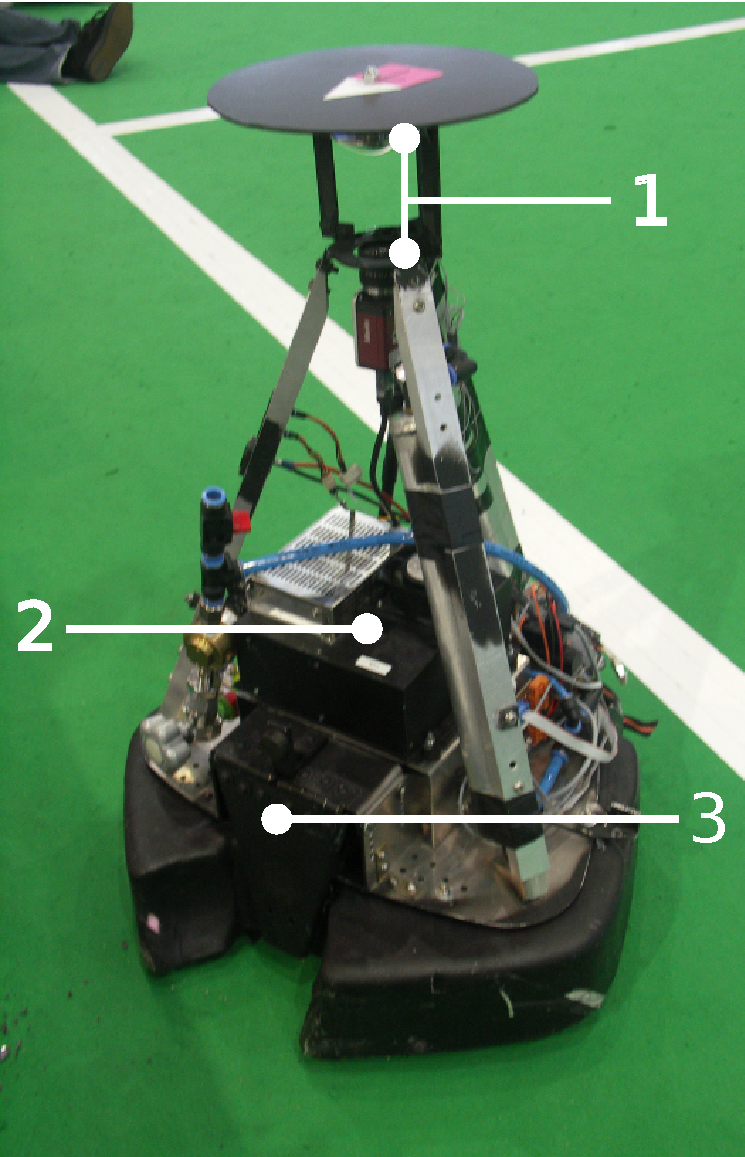
\includegraphics[width=0.5\columnwidth]{figures/krikkit.pdf}
\caption{\label{fig:krikkit}
Krikkit robot. Omni-vision with camera and mirror~(1); Industrial PC~(2); Pneumatic kicker~(3); Omni-drive is below the black bumper.
}
\end{center}
\end{figure}

It has a $360^\circ$ omnidirectional vision system via a firewire-camera pointing upwards to a hyperbolic mirror.\\
Its brain is a standard mini-ITX industrial PC.\\
A powerful pneumatic kicker, with a~200\,bar pressurised air bottle as supply, enables the robot to kick the ball approx.\ 10\,m forward.
The kicks are such powerful that the vibrations destroyed the former used hard disks now replaced by SSD~storage.
Additionally, every kick caused a camera blackout of nearly 2~seconds due to the vibrations.\\
Its drive system is also omnidirectional and is based on self-designed Mecanum wheels~\cite{mecanum2007}. 
The $45^\circ$\mbox{-}Arrangement of the wheels (see~\autoref{fig:mec-wheel}) promised smooth and vibration-free operation.
The three wheels are arranged in $120^\circ$\mbox{-}steps (see~\autoref{fig:omnidrive}) and are driven by a 200\,W brushless~DC motor for each axis.
Due to the nature of omni-wheels, the robots are able to move in any direction and any orientation.\\
The motors and all other electric components are supplied by a smart battery system~\cite{krammer06} with NiMH rechargeable batteries.
All electronic components are connected via CAN-bus.

\begin{figure}[htbp]
  \begin{minipage}{0.45\textwidth}
   \centering
    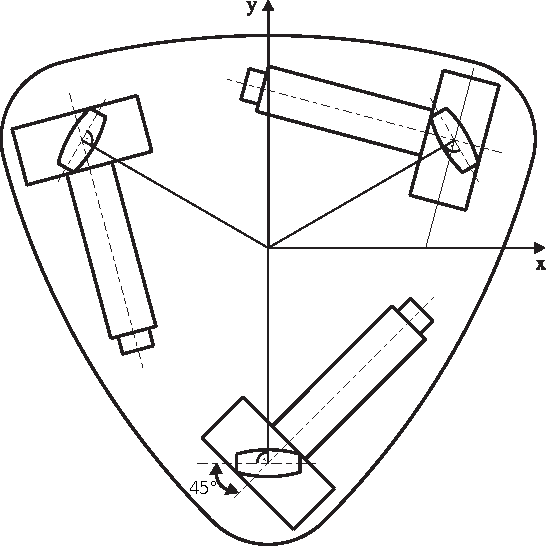
\includegraphics[width=1\textwidth]{figures/krikkit_drive_angles}
    \caption{\label{fig:omnidrive}Omni-drive schema of the Krikkit robot. The Mecanum wheels have their $45^\circ$~small wheels arranged in $120^\circ${-}steps around the centre.
    \cite{mecanum2007}}
  \end{minipage}\hfill
  \begin{minipage}{0.45\textwidth}
   \centering
    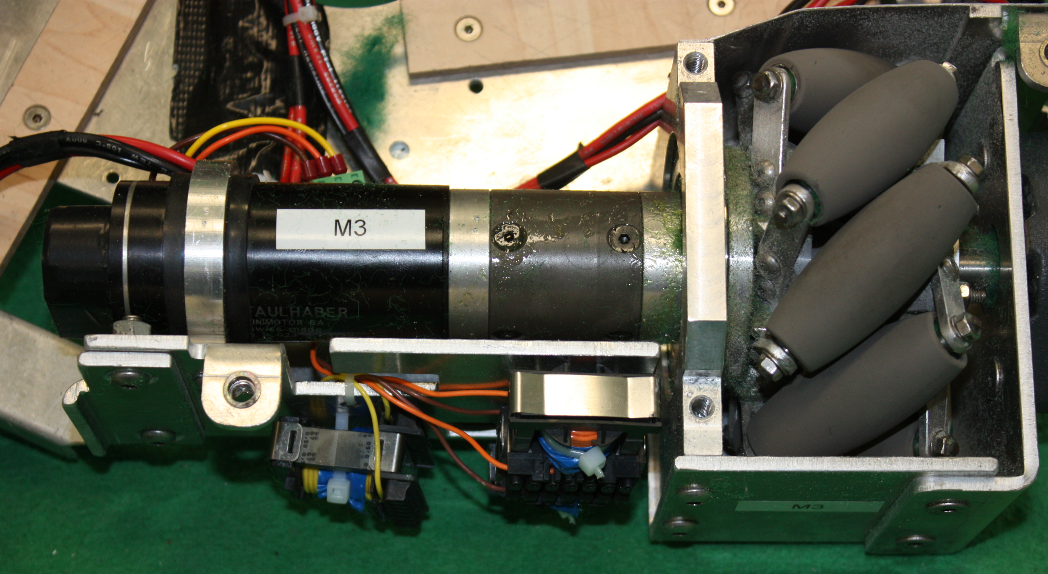
\includegraphics[width=1\textwidth]{figures/Omniwheel_drive.png}
    \caption{\label{fig:mec-wheel}Photo of one of the three Krikkit power trains, visible are from left to right: Motor, gearbox and Mecanum wheel.}
  \end{minipage}
\end{figure}


The Krikkit robots served well for four years and much was learned.
Before RoboCup~2009 in Graz a major mechanics overhaul was done.
In the meantime all major electronic components reached the end of their life cycle also.
With the knowledge gained, lost and acquired again the successor of the Krikkit generation is in development now.
    

\subsection{In Development: Krikkit3G}

The next generation of robots is in development since mid-2010.
It will be a direct successor of the Krikkit generation, therefore the name \emph{Krikkit3G}.

\Needspace*{4\baselineskip}
The successful concepts are adopted nearly unchanged:\nopagebreak[4] %% FIXXME only works inside sentences, want not to break up before the listing
\begin{itemize}
  \item omnidirectional drive with the three Mecanum Wheels
  \item the omni-vision system
  \item pneumatic kicking concept
  \item the use of a standard mini-ITX industrial PC
  \item modularity of all components
\end{itemize}

The new robot design focuses on the strict modularity of all components.
It has been shown that fast disassembling and replacing of critical components is crucial in the fast-paced tournament environment.
The power train has especially been modularised, the wheel, gearing, motor and motor electronics can be swapped as a whole group.

Tests showed that the smoothness of the Mecanum wheels had been insufficient due to manufacturing imprecision.
The resulting vibrations should be filtered out by an independent wheel suspension.

%  bumpers ?

For the kicking system the pneumatic principle was kept, but it is now much more versatile. 
It can switch between high and flat kicks at full power and side-kicks are also possible now.
Featuring a new ball guidance system allows grabbing the ball for a short moment.
This feature becomes especially useful when decelerating with the ball.
The vibrations from the kicker, disturbing the camera, should also be reduced by an active final position dampening system.
Nevertheless short disturbances in the vision system, due to the vibrations, will remain during the kicks.

Big changes have been made in the electronic sector.
A new microcontroller core (An ARM Cortex~M3) is used on every component, which replaces the different microcontroller architectures used before.
The smart battery system also got a major upgrade, featuring even smarter batteries.

In the mechanical design space is now also provided for an improved odometry system, which will be developed based on this work.

\begin{figure}[htbp]
\begin{center}  
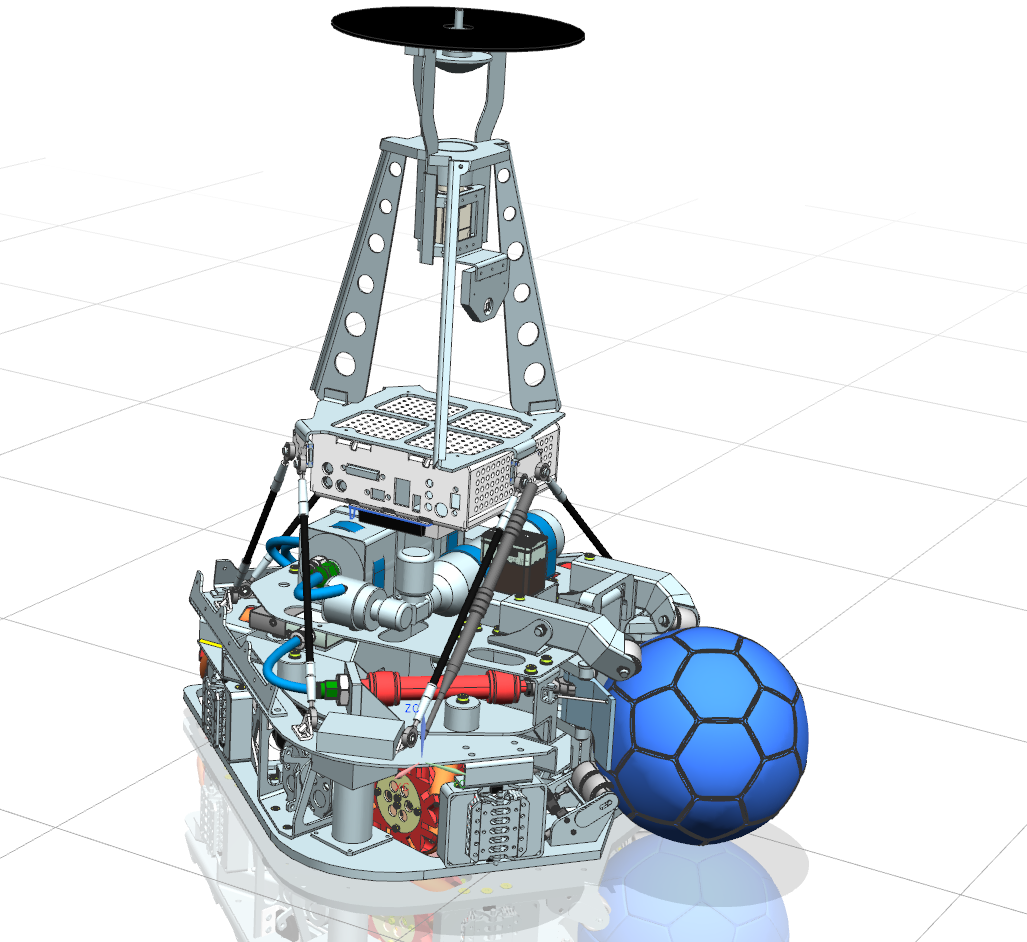
\includegraphics[width=0.7\columnwidth]{figures/Krikkit3G.png}
\caption{\label{fig:krikkit3g}
Rendering of the currently in construction Krikkit3G robot (Without outer hull).
}   
\end{center}
\end{figure}


% 1p

\subsection{Odometry}

%  Definition
%  Verwendungsmoeglichkeit
%    Lokalisierung
%      higher framerate than cam
%      backup-system for cam
%    Motion control
%      anti-slip regulation

Odometry, better known as path measurement is important for every moving vehicle, especially robots, which need to know where they currently are. 
The best known odometry measuring is used in cars as kilometre reading on the tachometer.

For autonomous mobile robots odometry plays an even more important role.
Together with the vision system and the compass it is a part in the sensor fusion for building the world model.
In the current Krikkit software, it fulfils the following purposes:
At first it acts as an initialisation vector for the vision system when comparing two camera frames for calculating the offset between them.
The second important role comes from the high frequency of odometry data.
Odometry data is provided with a frequency of 50\,Hz. 
This is much faster than the currently used vision system (15~-~25\,Hz). 
Therefore its values are added to the last known position in the world model for the time between two camera frames.
At last it acts as a backup system for the mainly vision based localisation system in case of camera blackouts e.g.\ blurred images due to the vibrations from a kick or a collision.

There are more possible use cases for odometry not implemented yet e.g.\ anti-slip regulation for every single wheel.



\subsection{Goals of this Work}
\label{motivation}
  
Current odometry systems of the Krikkit generation are based on the rotational speed of the wheels.
This has the major disadvantage of the accuracy being bound to the slip of the wheels. %FIXXME English being okay?
The problem is the non-uniform structure of the game field carpet, which has different slip factors in each direction.
Due to the different speeds and angles of the Mecanum wheels it leads to deviations even when driving a straight line.
The errors accumulate over time, resulting in $90^\circ$~deviation on 10\,m straight distance driven.

\Needspace*{4\baselineskip}
Therefore an wheel-independent odometry system has to be developed.
The goals of this work were:
\begin{itemize}
  \item Gathering requirements for a sensor
  \item Search for different types of sensors
  \item Implementation and validation of a prototype
\end{itemize}


\subsection{Requirements for a new type of odometry sensor on the Krikkit/3G platform}

The \MSL provides an ideal testbed for mobile robotics.
The main demands in robotics are miniaturisation, low cost, energy usage and robustness against the environment.

\Needspace*{4\baselineskip}
The range of application in the \MSL demands the following design parameters for an odometry sensor: %% FIXXME no page break here!
\begin{itemize}
  \item must deliver linear and rotational accurate data in three degrees of freedom
  \item must work on green carpet, other surfaces are bonus
  \item must not emit radiation or other disturbing effects irritating other robots or humans
  \item resistance against dust from the carpet abrasion
  \item shock resistant
\end{itemize}

The carpet is a particularly hairy concern, as its choice is up to the event organizer.
The only restriction in the \MSL rules and regulations~\cite{msl-rules} is: green.
Therefore the game field surfaces differ in colour and surface roughness on every event.
Colours from bright green over dark teal to nearly grey have been seen over the past years.
The roughness is another chapter.
It ranged from a very even felt with a roughness of maximum~2\,mm to an artificial grass like carpet with 15\,mm long hairs. 
Depending on the carpet the robot sinks in some millimetres, which also affects the clearance height.

The \MH requirements for a new odometry sensor are speeds of at least 5\,m/s at an operating frequency of at least 50\,Hz.
From the software side it would be highly appreciated if the sensor delivered data quality information.
Data quality information is crucial for the sensor fusion to recognize and de-prioritize erroneous data.
The \MH had bad memories about a malfunctioning compass ruining the world model.
At last the \MH has very tight budgetary limitations depending on external sponsors and due to being a student team.
The sensors have to be cheap enough to be affordable for series for up to six robots.


On the Krikkit3G robots the available space is limited to $50\times50\times110$\,mm$^3$ for each of the three proposed sensor mount points.
The Krikkit3G robot, similar to the old Krikkit generation, has a clearance height of 20\,mm.
Due to the new independent wheel suspension the operating range of the sensor must be in the range of $\pm 10$\,mm to the reference plane.
Data must be output on the robot's CAN-bus.
As power supply only two DC lines with 24\,V and 7\,V are available at reasonable currents.





\clearpage
\section{State of the Art in Odometry Measurement}

When determining the position or movement of a vehicle, there are the following options: 
Relying on global or relative position measurement.

The best known global position measurement is the Global Positioning System GPS.
This is widely used for robotics in outdoor applications where a GPS signal is available.
Indoors other known landmarks can be used.
In RoboCup the well-known shape of the soccer field is used for global reference.
Without exception every soccer robot uses the features of the game field e.g.\ the goals, lines and corner posts for orientation.\\
Other global approaches for gathering position data are compasses and gyroscopes.
They also deliver global data, but orientation and not position. 
This approach delivers only one of the three needed degrees of freedom, but it can complete the missing dimension.

% - global positioning
%   GPS
%   Compass
%   gyroscopes
%   relative position to known landmarks
%   - poles from 2006
%   - lines on the game field

For relative position measurement there is the choice to measure distance, velocity or acceleration.
Every approach has its advantages depending on the use case.
When aiming for the travelled distance it is not wise to measure acceleration, hence the measurement errors would sum up quickly due to the twice integration.\\
When measuring acceleration there is the choice between industrial grade accelerometers as used e.g.\ in aeroplanes and consumer grade accelerometers based on the piezoelectric effect.\\
Speedometers exist in various implementations based on the Doppler effect e.g.\ radar.\\
Distance metres can be mechanical or optical.
The simplest mechanical distance metre is a measuring tape, or when used on moving vessel, the log-line of a sailing ship used for speed measurement.
In the last decade another electronic approach was developed: optical distance metres based on comparing images for translational displacement, as used in optical computer mice.

% - relative positioning
%   - acceleration
%   - velocity
%   - distance
%   accelerometers
%   speedometers relying on the Doppler-effect
%   mechanical distance meters (like in cars or early computer mice)
%   optical distance meters based on comparing images for translational displacement, as used in optical computer mice


\Needspace*{4\baselineskip}
Every approach has properties to evaluate:
\begin{itemize}
  \item maximum and minimum speed capability
  \item maximum and minimum acceleration
  \item number of dimensions of movement data one sensor delivers
  \item linearity and deviation of data
  \item length of time of a single measurement
  \item time lag between measurement and data availability
  \item highest possible frequency of measurements
  \item resilience against reference surface distance changes
  \item maximum and minimum distance to reference surface
  \item surface state requirements
  \item resilience against environmental changes
  \item influence of the sensor on the environment 
  \item size and power requirements of the sensor
  \item cost of the sensors for three dimensions
\end{itemize}

In preparation for this work a lot of sensor types, both industrial and consumer grade, were evaluated for the use in the \MSL based on these properties.


\subsection{Possible New Odometry Sensors Types}

In this section technologies to be considered as improved odometry sensor are described in general.
The reasons for selecting a particular sensor type for evaluation in this work are explained in~\autoref{decision}.


\subsubsection{Accelerometers}

Accelerometers consists mainly of flexible mounted masses, which are under the influence of a force.
If the mounting consists of springs, the displacement is linear to an applied force.
This displacement is then measured.
Under normal circumstances on earth every object is under the influence of the gravitational force.
Therefore~1\,g must be subtracted from the result.

In commercial sensors piezoelectric elements are used to convert the force into a signal.
In the last years the use of micro electro-mechanical systems (MEMS) has been increased significantly.
Sensors for three dimensions are now available in tiny package formats at low cost for consumer applications.

\subsubsection{Gyroscopes}

Gyroscopes are inertial sensors, which detect the change of position.
Historically they consisted in a flywheel mounted in a Cardan suspension.
Once spinned up they remain at their orientation, based on the principles of conservation of angular momentum.

Today they are implemented as MEMS similar to  the before mentioned accelerometers.
Often they are even combined with accelerometers in a single chip package to 6-dimensional sensors.


\subsubsection{Ultrasonic Doppler velocimeters}

Ultrasonic Doppler velocimeters work similar as ultrasonic distance sensors.
Ultrasonic distance sensors were used in the first robot generation of the \MH for collision detection.

As on every Doppler measurement, its accuracy is directly dependant on the used wavelengths.
At ultrasonic sensors wavelengths around~100\,kHz are used. 
This leads to significantly more accuracy as e.g.\ Microwave Doppler sensors~\cite{ultrasonic}.

When working with ultrasonic sensors on mobile systems, one thing has to be taken into consideration: 
As on every wave-based system, the relative speed of the medium~(air) has to be considerably smaller than the wave speed ($v \ll c$).
Through the relatively low velocity of sound, only speeds up to~30\,km/h are feasible because of the head wind and turbulences~\cite{ultrasonic}.

Also, ultrasonic Doppler velocimeters subtle to vibrations due to low frequencies~\cite{agri}.

The main use today is in liquid flow measurements.



\subsubsection{Microwave Doppler Velocimeters (Radar)}

Radar is an umbrella term for object detection systems utilizing electromagnetic waves from 300\,MHz up to 3\,THz~\cite{nrt}.
It can be used to measure the distance of objects and also their speed through the Doppler effect.
Depending on the object distance, different wavelength are used.
For short-range measurements short-range microwave sensors with~24\,GHz are used e.g.\ radar guns and also for speed measurements on moving vehicles itself~\cite{s_r_radar}.

\subsubsection{Laser Interferometers}

Speed measurement with laser interferometry is divided into two approaches.
One called Laser Doppler velocimetry and the other is referred as Laser Doppler vibrometry.

In Laser Doppler velocimetry two coherent laser sources are intersected on the moving target surface at different angles.
The interference of the two beams creates a set of straight fringes. 
Particles of the surface, moving through the fringes, reflect light on the constructive interferences.
The resulting frequency is then captured by a photo diode~\cite{laser_vel}.

% source: WP

In a Laser Doppler vibrometer the beam is split into two coherent beams.
One beam is reflected and then interfered with the second beam and afterwards collected in a photo diode. 
The frequency shift between the two beams results in an overtone at the detector.

% source: WP

%\subsubsection{One-dimensional Optical Spatial Frequency Filtration}
%1/4



\subsubsection{Industrial/Custom-build Optical Speed Sensors}

The operation of an optical speed sensor is based on comparison of sequentially acquired images from a surface.
From the images, features are extracted, and their position is compared with similar features on the next frame. 

Such optical systems are common in industrial and consumer sensors.
Examplary uses are speed sensors for conveyor belts.

The components of an optical speed sensor are usually a high-speed camera, acquiring the images from the surface, and a Digital Signal Processor (DSP) for analysing the images.
In industrial systems the cameras are usually fixedly mounted and are connected to an external processing device~\cite{opt_vel}.

When the surface contrast is not sufficient to extract enough features for tracking, a little trick helps.
Every sufficiently rough surface creates a so-called \emph{speckle} when illuminated with a coherent light source.
This comes from the interference of reflected light waves with different phases due to the roughness of the surface.
Therefore illumination with a laser light source increases the contrast a lot on otherwise low contrast surfaces.
This is used e.g.\ in laser speckle strain measurement~\cite{strain}.

When developing such a system from scratch, a lot of time and effort is needed.
This has been shown by the development of an optical slip-angle sensor~\cite{Hrach2006} for the TUG~Racing~Team.

% 1/4
\subsubsection{Optical Mice}

The most common optical speed sensor is used in newer computer mice.
Historically computer mice featured a rolling ball with two attached axles (one for each axis), whose rotations are turned into coordinates.
In the last 10~years this mechanical principle has been superseded by a strictly electronic approach.

A standard optical mouse consists in a tiny camera taking images of the surface illuminated by an LED.
The processing of the images is done by an integrated DSP.
The sensor outputs movement data to an external microcontroller, which also handles the mouse buttons and translates all data to the~USB or PS/2 protocol.

At the time of the search~(2008), the fastest gaming mice had a maximum speed of 1.1\,m/s.\\
They operate at speeds up to 7\,000\,Hz.
Another advantage is their small size and minimal power requirement.\\
Being constructed as an exact gaming device also has disadvantages for RoboCup use:
To allow relocating the mouse very fast while lifting off, the best mice used for gaming are designed with a very short working range of only 2\,mm.

Laser mice use the same principle as the before mentioned laser speckle sensor.
The only difference to normal mice is the use of a coherent laser source as illumination instead of an LED.
The sensor itself remains the same, but due to the higher contrast achieved through the speckle, they work on more surfaces than common optical mice.

 
% 1/2

\subsection{Current Implementations used in RoboCup}

\subsubsection{\MH}

The current odometry system of the Krikkit robots is based on rotary encoders attached to each of the axles. 
The rotary encoders are needed for motion control, and odometry data fells off as a by-product.
The data from all three rotary encoders is collected by the motion controller, converted into $dr$,~$ds$,~$d\phi$ - coordinate values and send out on the CAN-bus.

Relying on the mechanical contact between the ground and the wheels brings various problems, as already mentioned in~\autoref{motivation}.
An effect known from all wheels is the slip on accelerating and braking.
The use of Mecanum wheels complicates the relationship between robot and the floor.
Due to different speeds of every wheel even when driving a straight line, resulting from the $120^\circ$\mbox{-}steps the wheels are mounted, every wheel has a different amount of slip.
Another factor not to be underestimated is the distinctive direction of the fibre of the carpets~\cite{mecanum2007}.
The direction of the fibre results in globally different friction factors in every direction.

Another common construction error of the power train used in the Krikkit robots was a loose connection between the gearing box and the motor.
The rotary encoders are mounted on the motors and not on the wheels.
When the connection between motor and the wheel got loose, the rotary encoders delivered only the rotation of the motor and not the distance covered by the wheels. 
This resulted in complete disorientation of the localisation software during an overrunning motor.\\
But faulty mechanics are not always responsible for this type of error, it is sufficient when a wheel looses contact with the ground for a moment.
This can happen when running aground on a lost screw or other parts lying around the game field or when two robots become wedged together.

For global positioning, in addition to the vision system, a compass is used.
Most of the time this works well, but once in a while we had problems with massive steel girders below the game field.
Due to the over-weighting of compass data, the localisation software went amok.
Therefore data quality information would be highly appreciated from every sensor used.

\subsubsection{Other Teams}

Rotary encoders on wheels are widely used, e.g.\ in the team ISocRob~\cite{isocrob}.
Other teams like IsePorto~\cite{iseporto} also accomplish the rotary encoders with a compass.

To counter at least the problem with the overrunning wheels when accelerating, e.g.\ the Iranian Team ADRO~\cite{adro} uses a second set of wheels for measuring odometry data.

The use of consumer computer mice in the \MSL has been tested by the Milan~Robocup~Team.
They used two optical mice mounted on the bottom of the robot.
The main advantages of this approach are the independence of the wheels and the low cost.
The availability of more dimensions than needed allowed for the corrections of non-systematic errors~\cite{two_mice}.

Accelerometers are used in other leagues, e.g.\ the RoboCup Rescue League or in the Standard Platform League with humanoid robots.
They are used only for inertial informations, not yet for navigation~\cite{zadeat}.


\subsection{Decision for a Type of Sensor}
\label{decision}

The focus lied on cheap consumer-grade sensor based solutions, due to the hefty price for industrial sensors.
Advantages of industrial solutions would be their robustness and in most cases their native CAN-bus interface.
But the big disadvantages of industrial sensors are the their size, weight and power requirements.
Finished industrial radars, laser interferometers and optical speeds sensors mostly use 230\,V~AC, require an external processing unit and are simply too big and heavy for middle size robots~\cite{laser_vel, opt_vel, s_r_radar}.

The approach of developing an optical sensor from scratch was shown to be successful for the automotive environment~\cite{Hrach2006}.
But it would need a lot of time and effort to shrink the gadget enough to fit inside a middle size robot.
At last, the components involving the camera and the needed FPGA-processor would be unaffordable for even one robot.

On ultrasonic sensors, most commercial sensors have $> $30\,cm surface distance, we have 20\,mm.
Reflections are another problem in ultrasonic measurement, we must use at least~3 sensors in close proximity to each other.
And due to the expected air turbulences close to the wheels as well as the reflection problem, the ultrasonic approach was rejected.

The main criterions against radar sensors are the very different reflection rates on different undergrounds (carpet, wood, concrete, steel, \dots).
The underground below the carpet is not known prior to a tournament, therefore the sensor is not guaranteed to work.
Other disadvantages are low accuracy at low speeds, and that radar is disturbed by nearby moving objects.

At time of search, consumer grade accelerometers/gyroscopes were not accurate enough to counter the summation errors.
An industrial Xsens~\cite{xsens} sensor would have better accuracy, but with a price tag of~\euro\,1.000 it was out of our budget.


The use of custom-build laser interferometers, especially vibrometers was considered.
The Institute of Electrical Measurement and Measurement Signal Processing does some work in this field.
The approach looked promising, but was not followed due to lack of time.

Mouse sensors were considered promising from the start of this project.
They are cheap, and fit into the size and power requirements of a middle size robot.
The disadvantages of missing range and maximum speed could be negated by replacing their optics.
By adding more magnification and setting the focus plane farther away from the sensor, maximum speed and range could be extended.\\
With the use of two sensors, the needed three degrees of freedom can be reached with extra redundancy. 
The \MH requires odometry data delivered on the CAN-bus, not the mice's native USB.
To convert four dimensions of data from two sensors into the needed $dr$,~$ds$,~$d\phi$ - values on the CAN-bus, a microcontroller controlling the two mice sensors is mandatory.\\
%The needed microcontroller-programming and skills in electrical measurement fit the telematics area ideally, so the approach with consumer mice with replaced optics was chosen.
%And last, but not least we got a sample mouse sensor sponsored from a friendly German RoboCup team, where an exhaustive data sheet was available~\cite{adns}.



%  entscheidung fuer einen Sensortyp
%    - why/why not...
%    - ...
%    - ...
%        2G spitzenvibration -> no

\clearpage
\section{Sensor Design}

The task is the following: Develop an odometry sensor from a given mouse sensor.
At the beginning of this project, we got a prototype sensor sponsored from (\$ German RC team FIXME).

It consisted of a mechanically modified Razor~Copperhead laser~mouse.
In this mouse type, a sensor from Avago~Technologies is used, the ADNS-6010.
The sensor and illumination were dismounted from its printed circuit board~(PCB) and relocated in a new casing because of mechanical size constraints (see~\autoref{fig:m-casing}.
It was reconnected to its PCB via thin enamelled copper wires.
It still worked, although the recommended distance to some circuit elements was exceeded considerably due to the 'extension' of the pins.

\begin{figure}[hb]
\begin{center}  
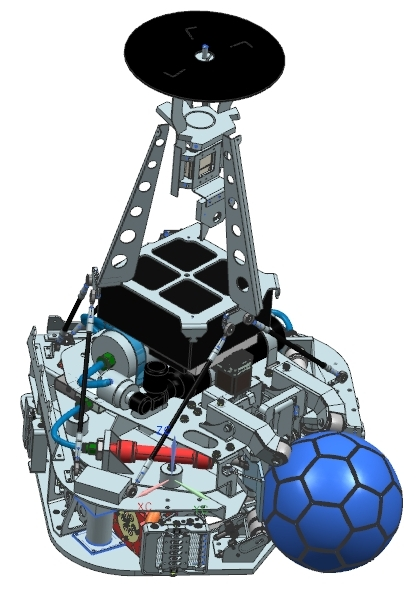
\includegraphics[width=0.5\columnwidth]{figures/Krikkit3G.jpg}
\caption{\label{fig:m-casing}
Prototype sensor from (\$ German RC team FIXME).
The Sensor~IC and the illumination was relocated from the PCB~(1) to an extension mount~(2).
}   
\end{center}
\end{figure}

Two modifications were to make: Providing a~CAN interface instead of USB, and creating a new optics system.
For the new optics system, access to raw sensor image data is needed for focussing the system.
Reading out raw image data is not possible via the mouse's USB interface, only directly via the SPI~(Serial Port Interface) of the sensor chip.
Therefore it was chosen to remove the sensor chip from the mouse, and connect it directly to an external microcontroller.
This kills two birds with one stone.
The microcontroller can provide a CAN-bus interface, and provides direct access to the sensor.\\
In summary, we have to create a system as shown in~\autoref{fig:block-diag-sens}.

\begin{figure}[hb]
\begin{center}
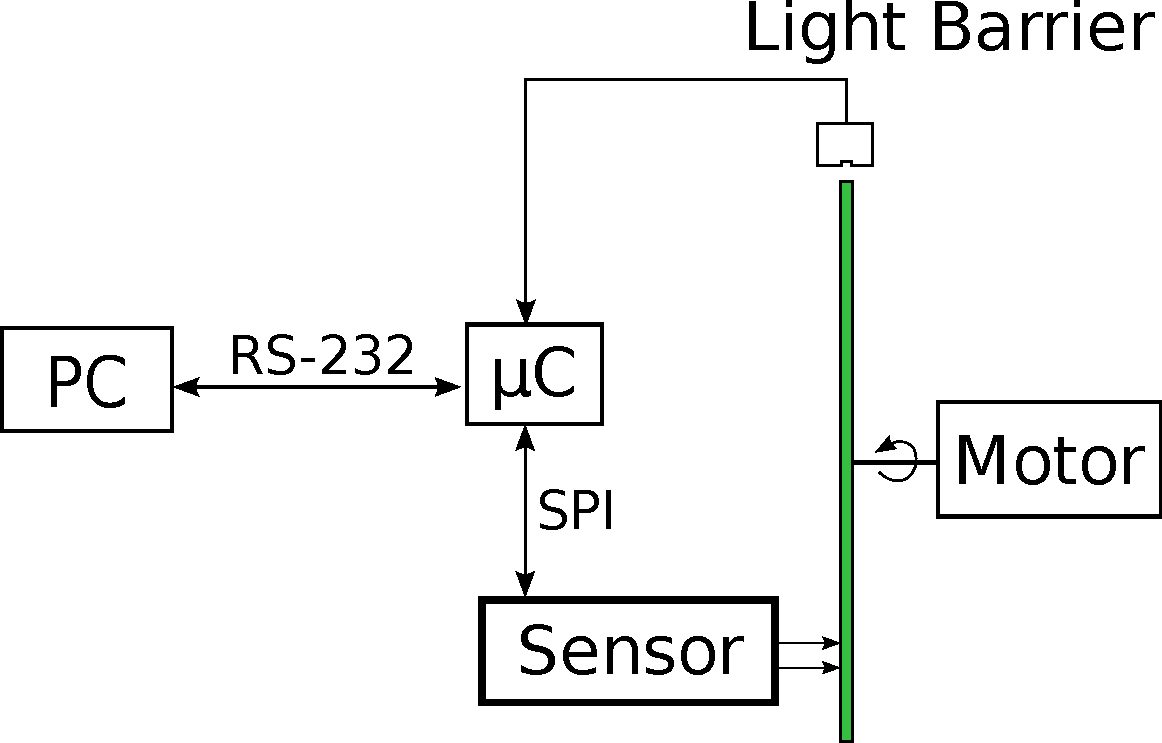
\includegraphics[width=0.9\columnwidth]{figures/block_diagram}
\caption{\label{fig:block-diag-sens}
Schemata of the sensor to be developed.
From left to right:
Optical system~(1) attached to the mouse sensor,
custom~PCB~(2) with the mouse sensor connected via SPI to microcontroller~(3), which is itself connected to a host~PC~(4) via serial~port~(RS-232).
The low level part of the software runs on the microcontroller, and the user interface runs on the host PC.
}

\end{center}
\end{figure}

We use an Infineon XC164-CM microcontroller evaluation board~\cite{xc}, of which several are available in the \MH.
For the mouse sensor, a custom PCB with minimal needed circuit and the needed connections to the microcontroller is designed.
The electronics part of this work is described in~\autoref{electronics}.\\
The Software part is split into low-level communication with the mouse sensor running on the microcontroller, and the controlling and visualising part on the host~PC, see~\autoref{software}.\\
The optical changes to the system with design and implementation are described in~\autoref{optics}.


\subsection{Electrical Design}
\label{electronics}

%Short text describing electrical layout

The ADNS-6010 laser mouse sensor runs on custom firmware, that must be flashed from the microcontroller to the sensor before motion read is possible.
Due to reluctant support from Avago Technologies, the firmware was not available as binary.
Therefore for connecting the microcontroller board with the ADNS-6010, two stages were needed.\\
The first stage features the microcontroller wire-tapping on the SPI channel between the original mouse microcontroller and the sensor, monitoring the communication, and recording the firmware as it is flashed on the sensor.\\
Now that we have the firmware, the sensor is unsoldered from the mouse PCB and inserted in a custom PCB with minimal needed circuit for communication with the new microcontroller.\\
In this subsection, at first the ADNS-6020 laser mouse sensor is introduced, then the XC164CM microcontroller and its development board.
At last, the needed circuit between the two chips for each stage is shown.


\subsubsection{ADNS-6010 Laser Mouse Sensor}

The ADNS-6010 laser mouse sensor measures changes in position by optically acquiring sequential images and mathematically determining the direction and magnitude of movement.
It contains an image acquisition system, a Digital Signal Processor~(DSP), and a four wire serial port.
It acquires microscopic surface images via the lens and illumination system. 
These images are processed by the DSP to determine the direction and distance of motion. 
The DSP calculates the $\Delta x$ and $\Delta y$ relative displacement values. 
The $\Delta x$ and $\Delta y$ values are output on the serial port to an external microcontroller.~\cite{adns}

%workflow diagram (from data sheet) (none found?)
 
It features the following specifications:
\begin{itemize}
 \item High speed motion detection –- up to 1100\,mm/s and 20\,g
 \item Programmable or automatic frame rate over 7080 frames per second
 \item 400, 800, 1600 or 2000\,cpi selectable resolution
 \item Single 3.3\,V power supply
 \item Four-wire serial port along with power down, and Reset pins
 \item Integrated laser driver controller for illumination laser diode
\end{itemize}

It comes in a 20-pin package, bundled with its own lens and matching vertical-cavity surface-emitting laser diode (VCSEL).
It uses 3.3\,V, but can be connected to a 5\,V-microcontroller without level shifting techniques needed.
The data connection to the microcontroller is a four-wire serial port interface (SPI).
The lines are source clock (SCLK), chip select input (NCS) which activates the SPI, and the in (MOSI, Master Out/Slave In) and out (MISO, Master In/Slave Out) data lines.
The microcontroller acts as master and always initiates the data transfer.\\
Some additional circuit, e.g.\ external reference capacitors and a resonator is needed, as shown in~\autoref{fig:adnsc}.

\begin{figure}[htbp]
\begin{center}  
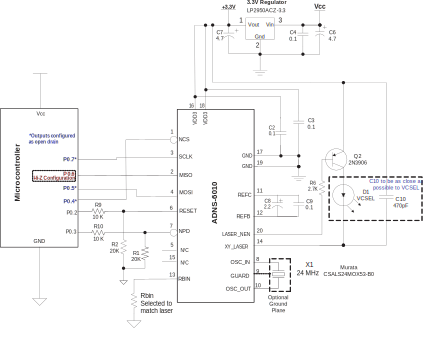
\includegraphics[width=1\columnwidth]{figures/adnsc}
\caption{\label{fig:adnsc}
Minimal circuit for the ADNS-6010 laser mouse sensor recommended from data sheet~\cite{adns}.
The ADNS-6010 is in the centre, the external microcontroller on the left side, the VCSEL laser and driver on the right.
The 3.3\,V-regulator needed on 5\,V supply is on top of the diagram.
}   
\end{center}
\end{figure}


\subsubsection{XC164CM Microcontroller}

The XC164CM microcontroller comes from the Infineon XC166 family, as used in the Krikkit robots for motion control~\cite{krammer07}.
It is a 16-bit microcontroller, which allows for convenient programming via the Keil\footnote{Keil uVision3 V3.30a \copyright~Keil Software Inc.\ downloadable from: \url{http://www.keil.com}}~IDE.\\
A XC164 development board~\cite{xc}, as seen in~\autoref{fig:xcdevboard} is used. 
It has all pins of the XC~core easily accessible, and all needed circuit for the XC is on board.
The XC164 on the board runs on 5\,V supply, which is tapped to power the ADNS-6010.
The use of an oversized evaluation board is of course no option on the Krikkit/3G robots, but sufficient here.

\begin{figure}[htbp]
\begin{center}
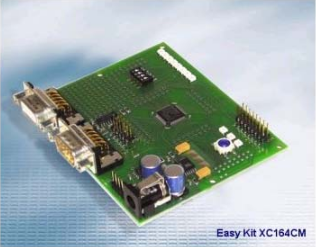
\includegraphics[width=0.5\columnwidth]{figures/xcdevboard.png}
\caption{\label{fig:xcdevboard}
XC164CM development board~\cite{xc} used to control the sensor.
It needs 12\,V external power supply (connector visible on the bottom).
It has external RS-232 (left) and CAN (middle) connectors.
}
\end{center}
\end{figure}

For development, the microcontroller board is connected via its serial port (RS-232) to a host computer.
Programming as well as controlling and reading out data is done over the serial port.
The CAN interface of the microcontroller is only needed on the final implementation on the robot, therefore it is not connected at the moment.\\
For connection to the ADNS-6010, a 10-pin header is soldered subsequently on the development board and connected to the needed pins of the XC core~(see~\autoref{fig:boardwiring}).
Besides the 4-port SPI, reset and power down (NPD) lines and the power supply (VCC and GND) are intended for the ADNS-6010.
Then it is connected via a ribbon cable to the original mouse PCB for wire-tapping (Stage~1) and later to the new ADNS sensor board (Stage~2).
The pin-assignment of the header and cable can be seen in~\autoref{pin-table}. 

\begin{table}[htbp]
  \begin{minipage}{0.55\textwidth}
    \centering
    \begin{tabular}{|l|l|l|l|}
       \hline
       Pin & Name & XC Port & PCB Con\\
       \hline
       1    & NCS   & P3.6  & X107.1     \\
       2    & MISO  & P3.8  & X107.3     \\
       3    & SCLK  & P3.13 & X107.7     \\
       4    & RESET & P9.4  & X107.15    \\
       5    & MOSI  & P3.9  & X107.4     \\
       6    & N/C   & -     & -          \\
       7    & NPD   & P9.5  & X107.16    \\
       8    & N/C   & -     & -          \\
       9    & GND   & -     & X107.9     \\
       10   & VCC   & -     & X107.8     \\
       \hline
    \end{tabular}
  \end{minipage}\hfill
  \begin{minipage}{0.45\textwidth}
    \centering
    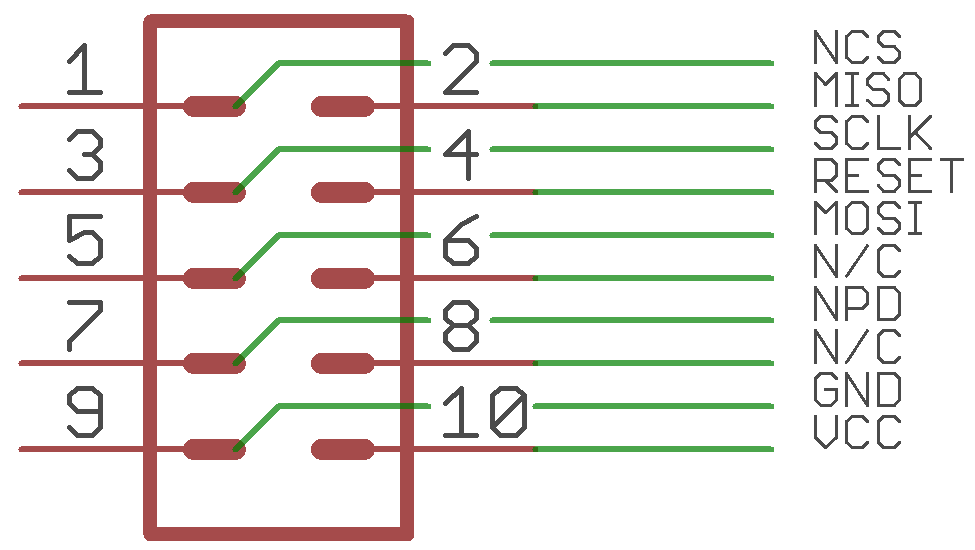
\includegraphics[width=1\textwidth]{figures/header.png}
  \end{minipage}
  \caption{Pin-assignment of the 10-pin header and cable on the XC164CM development board.}
  \label{pin-table}
\end{table}

\begin{figure}[htbp]
\begin{center}
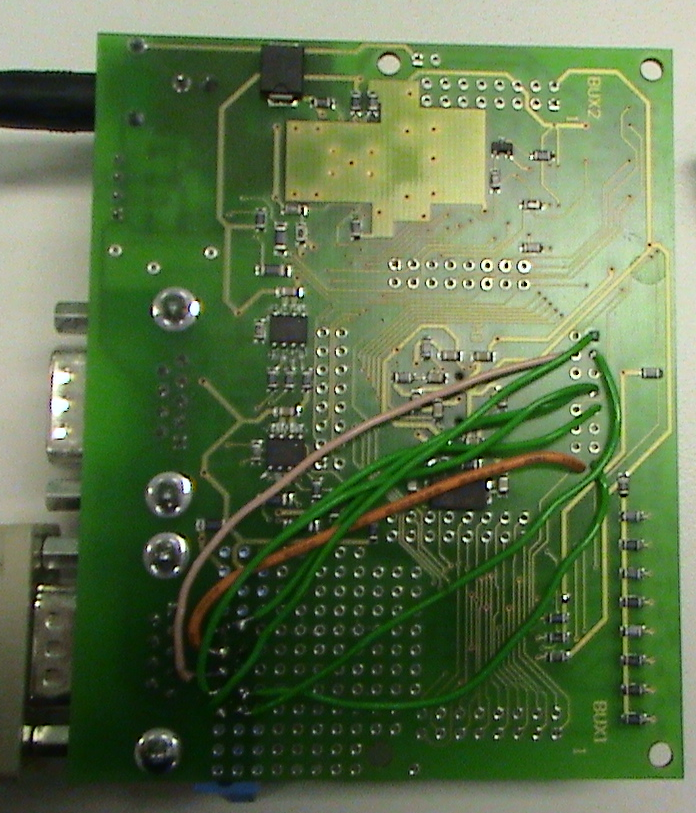
\includegraphics[width=0.5\columnwidth]{figures/boardwiring.png}
\caption{\label{fig:boardwiring}
%FIXME newer pic with measurement bridge
Wiring of the XC164CM development board.
The pins from the XC are connected from the header X107 (middle right) to the 10-pin header (lower left) and the measurement bridge (lower right).
}
\end{center}
\end{figure}


The second role of the XC board is the reference speed measurement on the experimental set-up via a light barrier.
The circuit and function of the needed measurement bridge is described in~\autoref{lb}


%Specs etc

%XC-164 eval board 
%  Image from datasheet

%Wiring of the Evaluation Board

%  block diagram

%  circuit
    


\subsubsection{Wire-tapping Circuit for Firmware Catch}

%Beschaltung beschrieben

The goal in stage~1 is to catch the firmware written from the mouse microcontroller to the ADNS-6010 for ourselves use.
The firmware must flashed after powering up the mouse to the ADNS-6010.
After powering up, the reset pin of the ADNS-6010 is toggled by the mouse microcontroller, and directly after that event the control sequence for downloading to the SROM starts, followed by the firmware.
The idea is to connect the XC as a second slave to the bus, and record all communication between the mouse microcontroller and the ADNS from the moment the reset pin is toggled.
We need only four lines: GND, RESET and from the data interface only SCLK and MOSI. 
The SCLK is needed, because SPI works as a synchronous interface, and we do not know the exact frequency of operation.
We only need the data written from the microcontroller to the ADNS (MOSI), the reverse channel is uninteresting.\\
In the implementation four wires are soldered on the GND, RESET, SCLK and MOSI pins of the mouse, and connected via a crimp plug (pin assignment see~\autoref{pin-table}) to the 10-pin header on the microcontroller development board. 
This set-up can be seen in~\autoref{fig:wiretapping}.

\begin{figure}[htbp]
\begin{center}
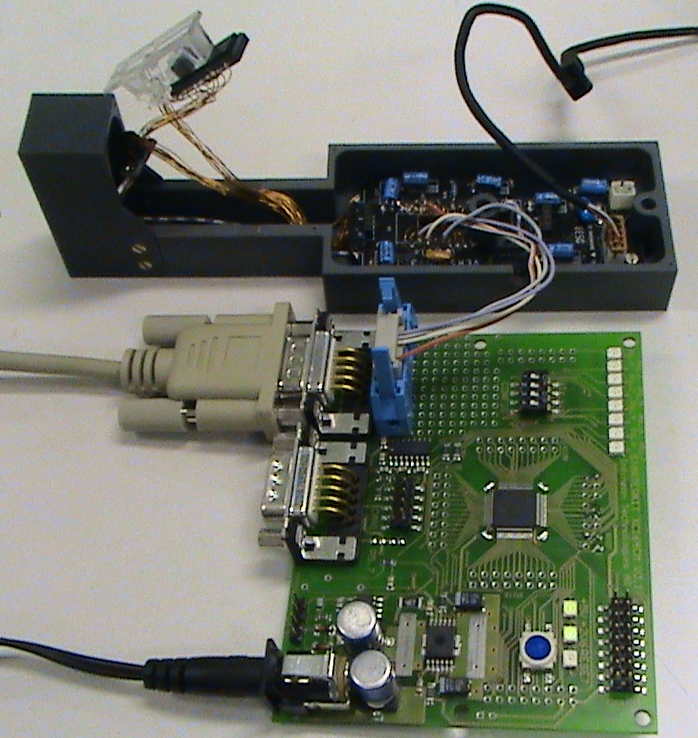
\includegraphics[width=0.8\columnwidth]{figures/wiretapping.png}
\caption{\label{fig:wiretapping}
Implementation of the wire-tapping to catch the firmware (stage~1).
On top is the mouse, with the sensor on its original PCB.
The four needed lines GND, RESET, SCLK and MOSI are connected to the microcontroller development board (bottom).
Our microcontroller is configured as slave and waits for the reset signal, after which the communication between mouse microcontroller and ADNS on the SPI is monitored, and the firmware recorded.
}
\end{center}
\end{figure}

% 4x vorgang kommt zu uC-software

\subsubsection{Final Circuit between ADNS and XC}
\label{adns-pcb}

After successfully saving the firmware in stage~1, we can connect the ADNS-6010 directly to our microcontroller.
With the outputs of the XC164CM configured as open drain, we can connect the 5\,V microcontroller with minimal circuit to the 3.3\,V~ADNS-6010.
The ADNS-6010 is mounted on a custom PCB with the following features: 
10-pin header for connection to the microcontroller board,
\hbox{3.3\,V-regulator},
circuit needed for the VCSEL diode,
resonator and reference capacitors.\\
The board layout is designed in the Cadsoft EAGLE\footnote{EAGLE light edition v5.10.0 \copyright~CadSoft, \url{http://www.cadsoft.de} as on 1/1/2011} Software.
The EAGLE-files are available in the AFS\footnote{/afs/robocup.tugraz.at/electrics/design/99\_concepts/adns\_testplatine/v1.1 as on 21/12/2010}.
The circuit and board layout for the PCB can be seen in~\autoref{fig:testplatine-layout} and~\autoref{fig:testplatine-board}.

\begin{figure}[htbp]
\begin{center}
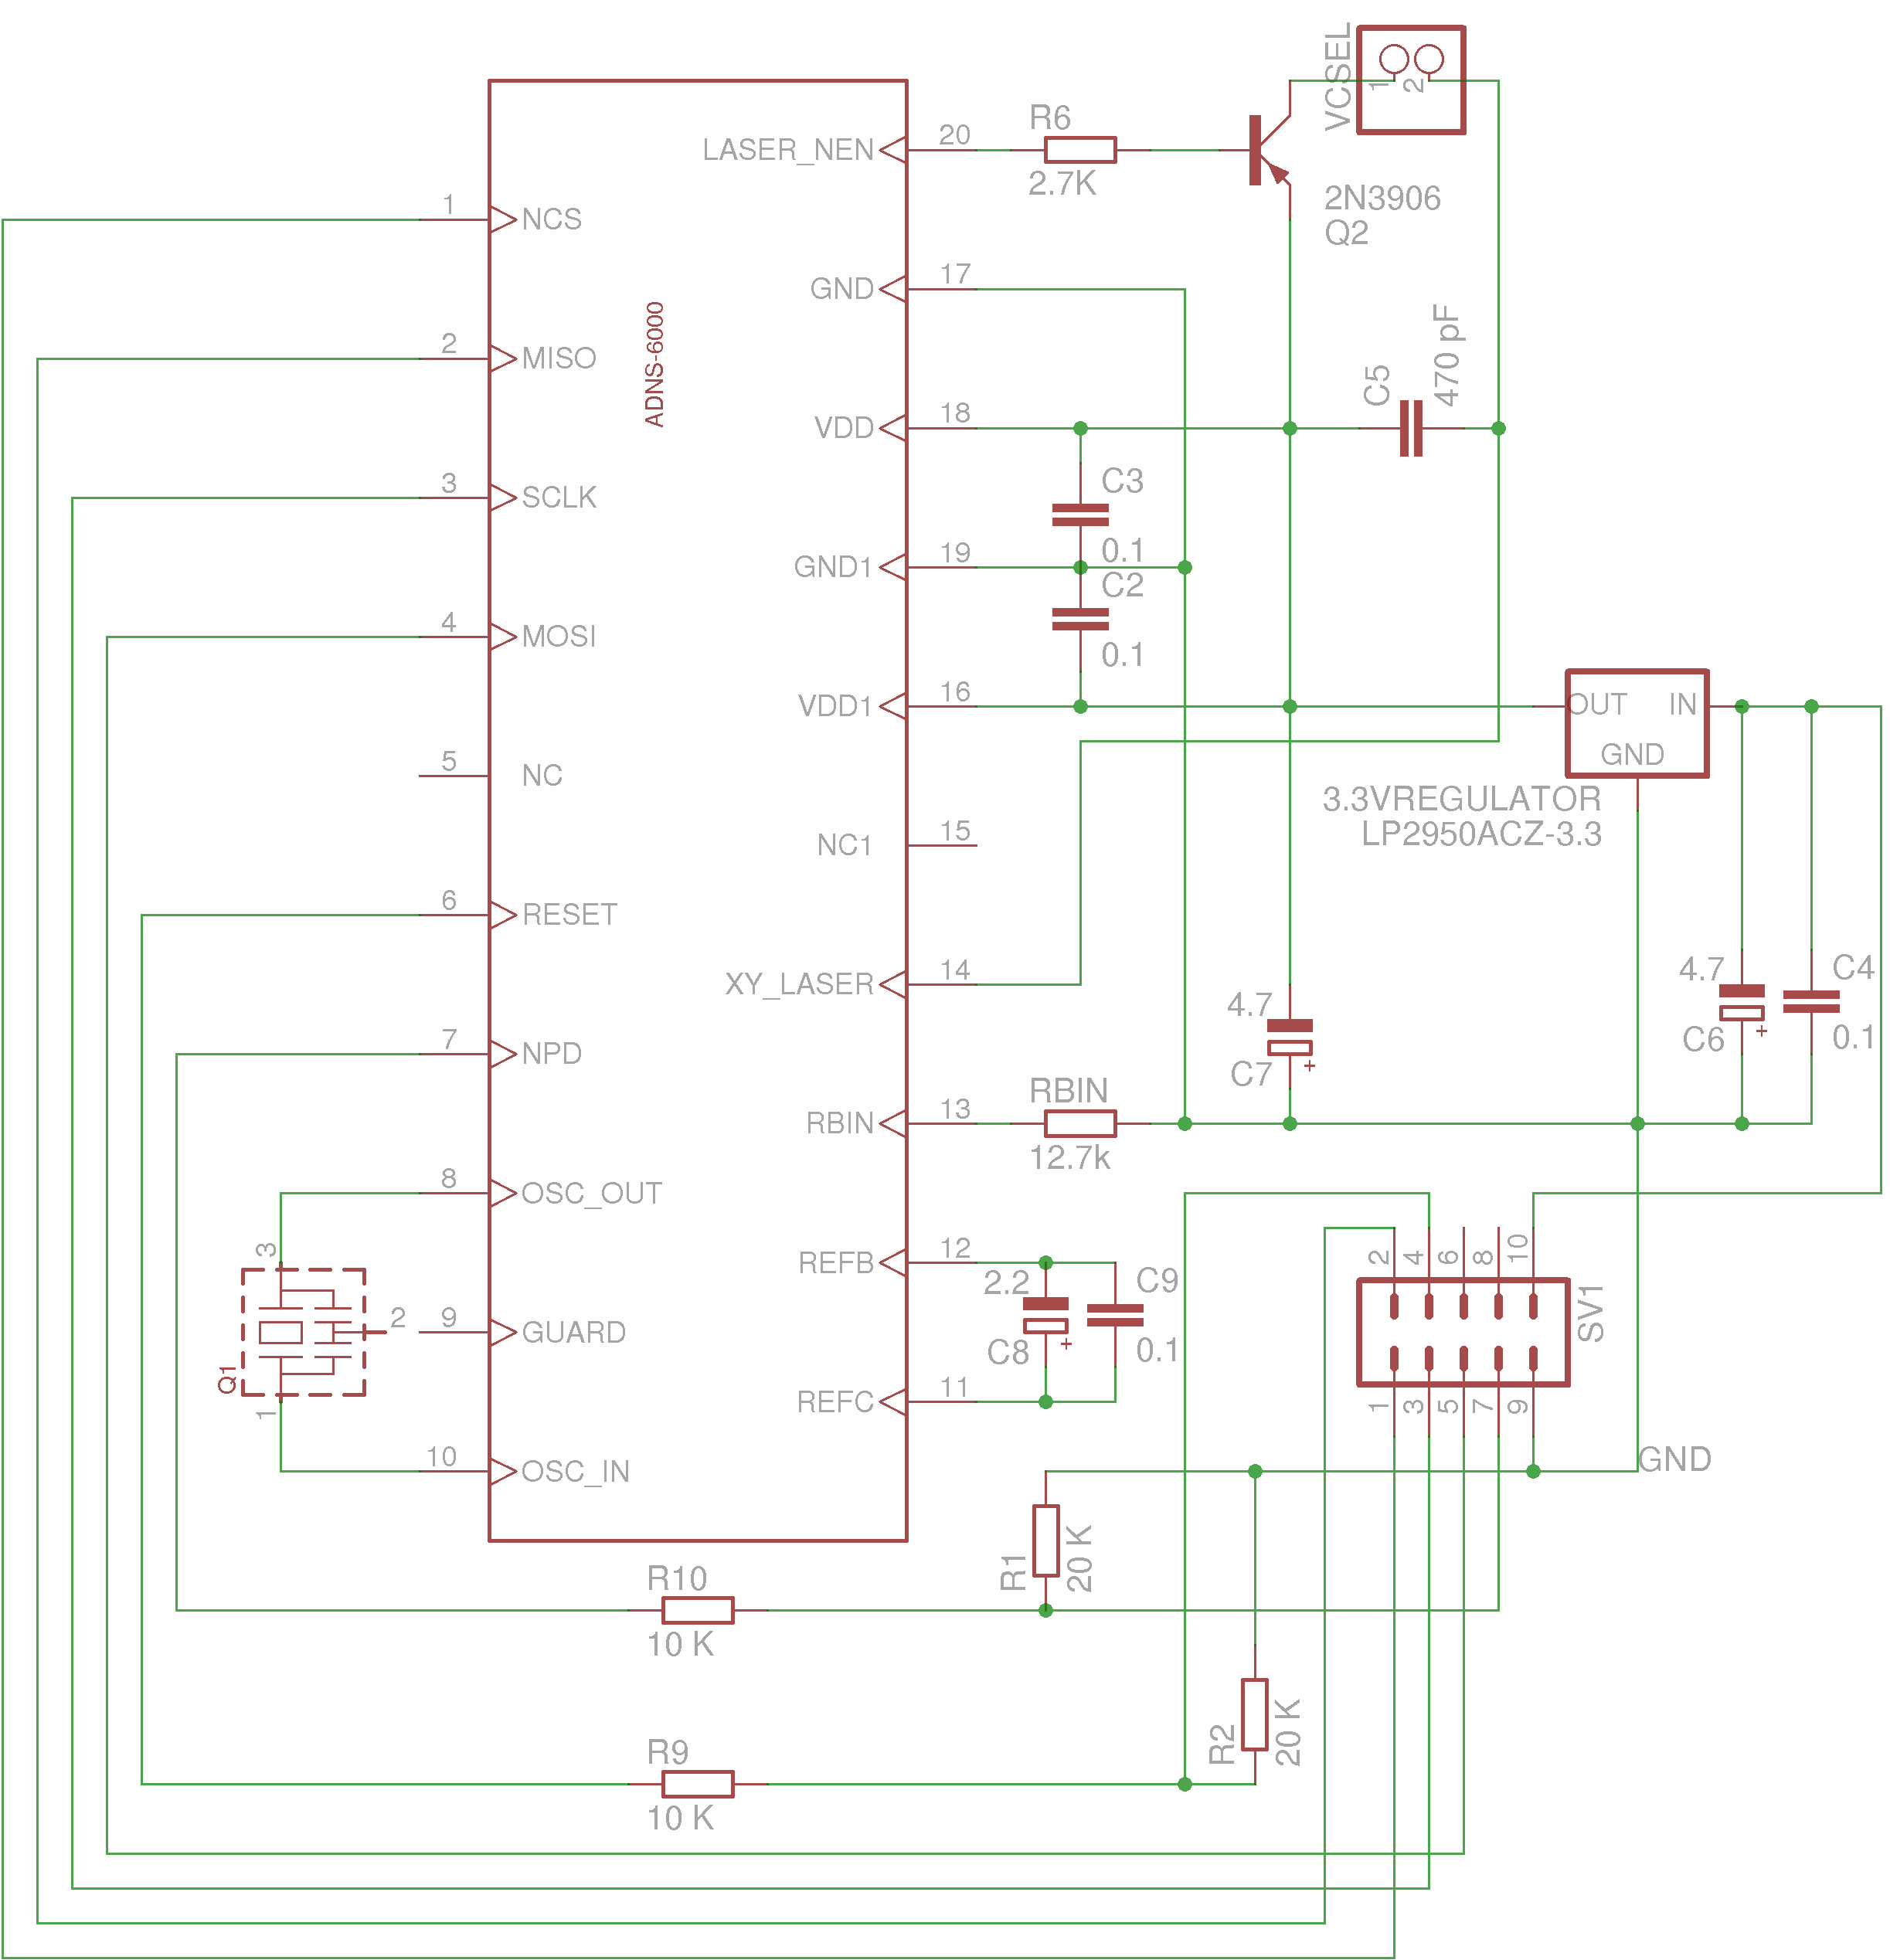
\includegraphics[width=1\columnwidth]{figures/schaltplan.png}
\caption{\label{fig:testplatine-layout}
Circuit for the custom PCB for the ADNS-6010 laser mouse sensor.
In the lower right is the 10-pin header for the connection to the microcontroller board.
Right on the middle the 3.3\,V-regulator, which takes it power from the 5\,V-line from the microcontroller.
Top right is the header for the externally connected laser diode.
}
\end{center}
\end{figure}

\begin{figure}[htbp]
\begin{center}
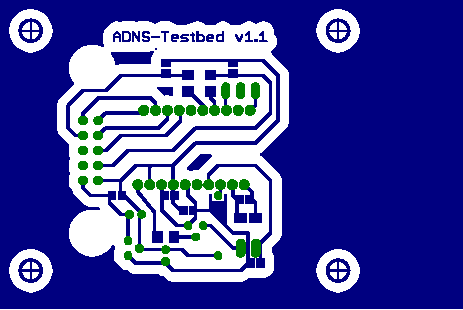
\includegraphics[width=0.5\columnwidth]{figures/platine}
\caption{\label{fig:testplatine-board}
Board layout for the custom PCB for the ADNS-6010 laser mouse sensor.
The 20-pin sensor is in the middle.
On the left is the 10-pin header for the connection to the microcontroller board.
Below the sensor is the 3.3\,V-regulator, and driver and header for the externally connected laser diode.
Sketch not to scale.
}
\end{center}
\end{figure}

\subsection{Optical System}
\label{optics}

%requirements
%  surface distance from 2mm to 20mm
%  5x magnification
%  telecentric optical path

The optical properties of the mouse have to be improved by an appropriate optical system.
The most important drawback of the ADNS-6010 is its maximum capable speed of 1.1\,m/s, it must be improved to 5\,m/s. 
The maximum speed is linear dependant of the field of view of the sensor.
By magnifying the field of view of the sensor by five times, this will also increase the maximum speed over 5\,m/s.\\
Another wished feature is a distance to the surface from at least 20\,mm.
The ADNS-6010 with its original lens has only 2\,mm clearance height, this has to be improved.\\
And due to varying clearance height resulting from the new independent wheel suspension as well as different carpets, the dependency of the magnification from the clearance height should be eliminated.
This can be achieved by a telecentric system~\cite{telec}.

It is chosen to keep the original lens in its position, and extend the optical system with additional lenses.
At first, a lens is added in front of the original lens, which provides the needed magnification.
Then, a second lens is added responsible for the telecentric set-up.
We call the original mouse lens L$_1$, the magnification lens L$_2$, and the telecentric lens L$_3$. 
The aperture stop of the system responsible for the sharpness of the image is placed at L$_2$.
The whole optical system can be seen in~\autoref{fig:sketch-optic-simple}.

\begin{figure}[htbp]
\begin{center}
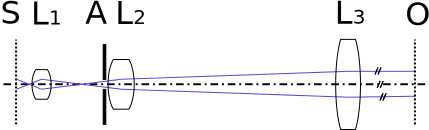
\includegraphics[width=1\columnwidth]{figures/sketch-optic-simple}
\caption{\label{fig:sketch-optic-simple}
Complete optical system:
Image plane~S on the left side,
original mouse lens L$_1$,
aperture stop~A,
magnification lens~L$_2$,
telecentric lens~L$_3$ and object~O on the right side.
}
\end{center}
\end{figure}
%Sketch

The optical system with the sensor is built using a Linos 40\,mm micro-bench carrier system~\cite{microbench} which allows for easy adjustment of all optical components.
For some of the components a custom mount based on micro-bench carriers has to be developed, so for L$_2$ and the aperture, due to space constrains (see~\autoref{l2m}).
The mount of the sensor itself on the micro-bench carrier is described in~\autoref{semo}.

The calculations involved figuring out the original mouse optical system, designing the second lens and needed aperture and choosing an appropriate lens for the telecentric set-up.
All calculations are verified with WinLens3D\footnote{Qioptiq Photonics GmbH \& Co.\ KG, WinLens3D Basic V1.1.11, \url{http://www.winlens.de} as on 30/12/2010} and are available in the AFS\footnote{/afs/robocup.tugraz.at/projects/2010\_improved-odometry/lenses/ as on 30/12/2012}.
Detailed explanations of the calculations follow now.

\subsubsection{Optical Path Calculations: Original Mouse Setup}

To alter the properties of an optical system by expansion with more optical elements, the optical properties of the base system must be known.
The original mouse sensor set-up consists of the sensor, the lenses for the sensor and the VCSEL combined as one plastic part, and the VCSEL (see~\autoref{fig:o_setup_datasheet}).
The exact parameters of the optical system are not specified in the data sheet, they have to be estimated based on retroactive measurements and own observations.
From the data sheet~\cite{adns} the following properties are known: 
\begin{itemize}
  \item Distance of sensor plane to lens plane is 5.88\,mm.
  \item Distance from lens plane to object plane is also 5.88\,mm.
  \item The lens material has a refraction index of $n=1.5713$ at $\lambda=842$\,nm.
  \item Lens thickness is 2.43\,mm.
\end{itemize}

\begin{figure}[htbp]
\begin{center}
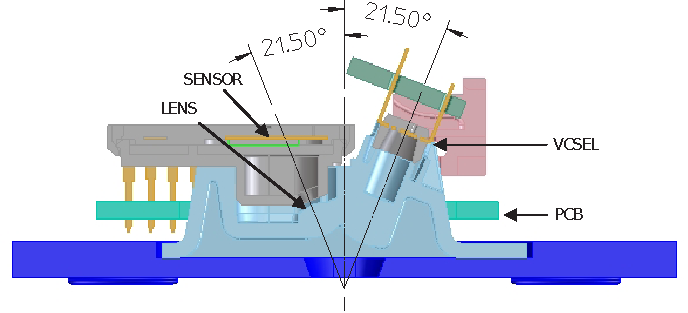
\includegraphics[width=1\columnwidth]{figures/o_setup_datasheet}
\caption{\label{fig:o_setup_datasheet}
Original mouse set-up from the data sheet~\cite{adns}.
The optical rays from the VCSEL~(right) and the sensor~(left) meet on the surface.
}
\end{center}
\end{figure}

With these informations, we can estimate a focal length of 2.88\,mm for the original mouse lens.
With the distance of the sensor and object plane being the same of both sides of the lens, this leads to a magnification factor of~1.
The measured aperture diameter (of the hole in the chip casing) on the original lens is~1.4\,mm.
The sensor delivers a quadratic image with a side length of approx.~0.92\,mm. 
Therefore we get a maximum image size of 1.3\,mm diameter.\\
These findings were confirmed by the simulation via WinLens.
The WinLens sketch of the system can be seen in~\autoref{fig:ls1_p}.
The according spot diagrams are satisfactory, see~\autoref{fig:ls1_s}.
The simulation is done for $\lambda = 842$\,nm, the wavelength of the illuminating VCSEL. 
The modelling of the first lens is used as base for the simulation of the extended optical systems in WinLens.

\begin{figure}[htbp]
\begin{center}
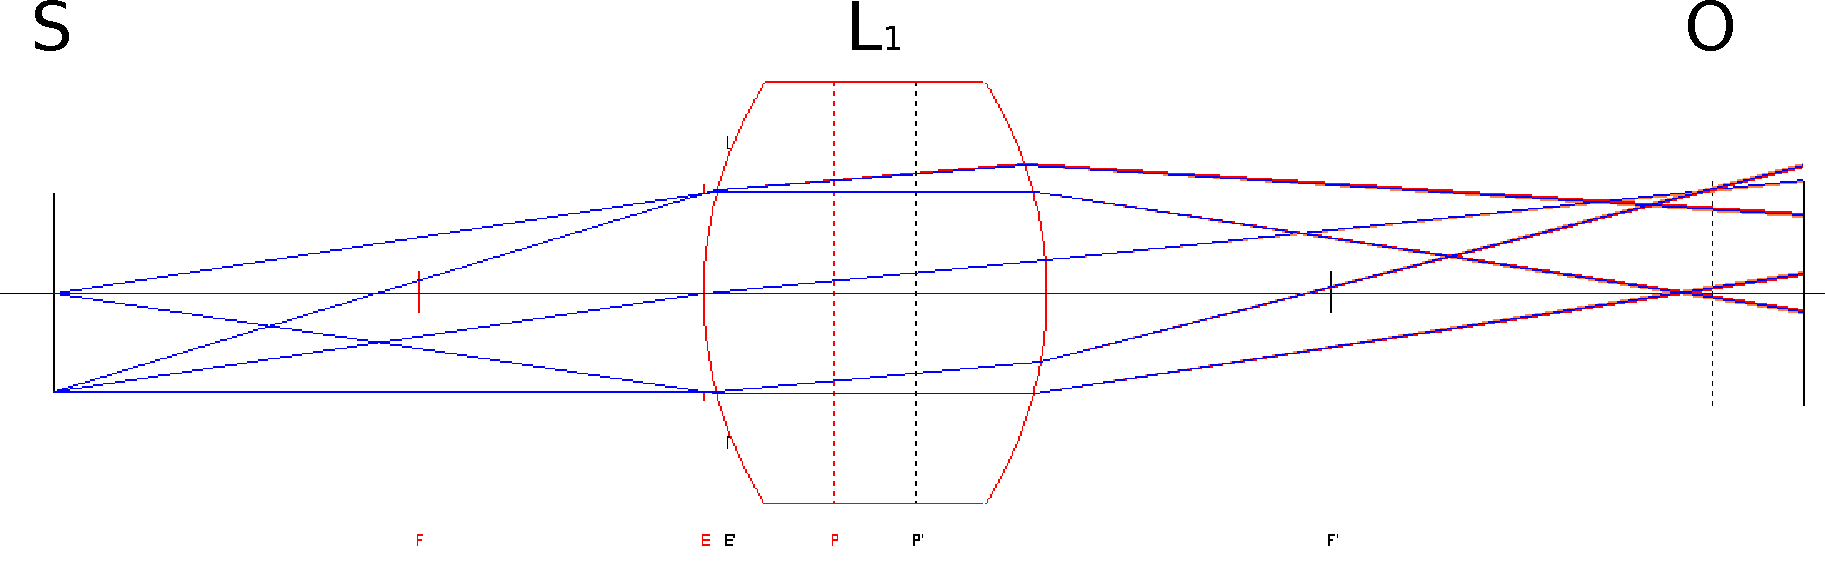
\includegraphics[width=1\columnwidth]{figures/lens_system_mouse.pdf}
\caption{\label{fig:ls1_p}
WinLens plot of the simulation of the unmodified optical system of the mouse.
One single lens with $f=2.88$\,mm sits exactly in the middle between sensor plane~S and object plane~O.
}
\end{center}
\end{figure}


\begin{figure}[htbp]
\begin{center}
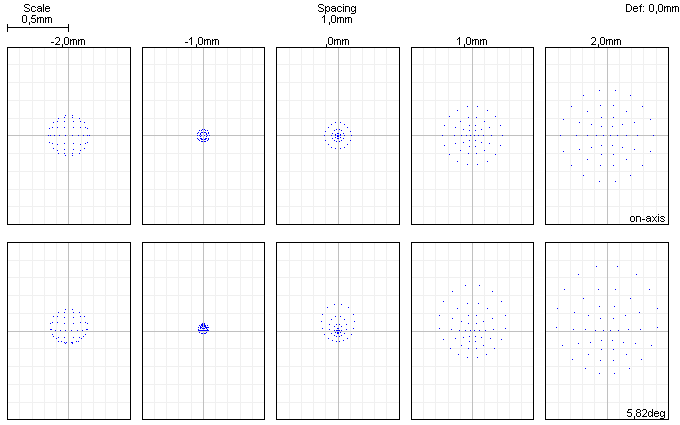
\includegraphics[width=1\columnwidth]{figures/spot_diagram_mouse.png}
\caption{\label{fig:ls1_s}
WinLens plot of the spot diagram of the simulation of the unmodified optical system of the mouse for $\lambda = 842$\,nm.
The focusing of the spots hint to a relatively well modelled system.
}
\end{center}
\end{figure}

\subsubsection{Optical Path Calculations: 2-Lens Setup}
\label{opt:2l}

The goal is to find a lens set-up that magnifies the current optical system by five times.
We design the system without telecentric at first, as a telecentric add-on does not alter the magnification of the system.
For a magnifying system, we add a second lens before the original system that has its image plane on the object plane of the original system (see~\autoref{fig:sk2l}).
The needed focal length $f_2$ of lens~2 is calculated from the Laplace projection equation~\cite{jaeger}:% (\autoref{eq:1}). %FIXME auf deutsch heissts so, wie in EN-GB? (nur thin lens eq. gefunden, das is net das was wir schreiben wollen)

\begin{equation}
\label{eq:1}
\frac{1}{f_2} = \frac{1}{o_2}  + \frac{1}{i_2}
\end{equation}

$o_2$ is the object distance, $i_2$ the image distance from the lens.
We want to set $o_2 = 5 \cdot i_2$ for a magnification factor of five.
From the range of possible values for $o_2$, we are limited by the maximum available space for the odometry sensor in the robot.
The extension of the optical system must be at most 80\,mm long, therefore $o_2$ should be no longer than 65\,mm.

\begin{figure}[htbp]
\begin{center}
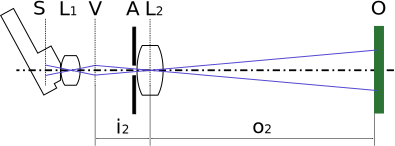
\includegraphics[width=1\columnwidth]{figures/sketch-optic-2lens}
\caption{\label{fig:sk2l}
Sketch of the extension of the original system with a second lens.
From left to right: 
Sensor plane~S,
original mouse lens~L$_1$, 
virtual image plane~V (former object plane),
second lens~L$_2$ with new aperture~A and
new object plane~O.
Dimensioning below are: 
Image distance~$i_2$ to virtual image and object distance~$o_2$ for magnifying lens~2. % FIXME cite? from WP... but need better ref.
}
\end{center}
\end{figure}

The next criteria for the lens system is the depth of focus.
We wish for $\pm 10$\,mm depth of focus to the object plane.
For any symmetrical lens, the depth of focus lies between the near and far limits, see~\autoref{fig:nfl}.
\begin{figure}[htbp]
\begin{center}
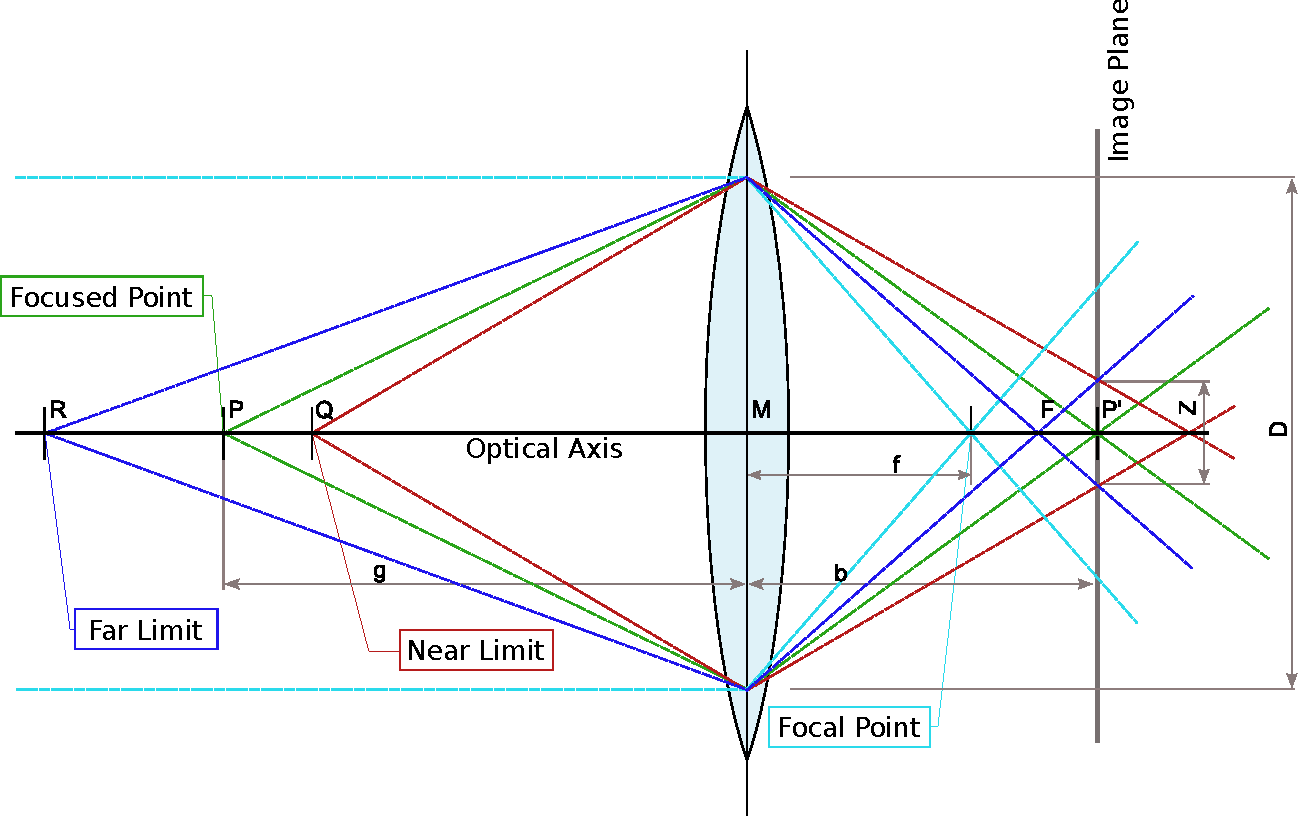
\includegraphics[width=1\columnwidth]{figures/near_farpoints}
\caption{\label{fig:nfl}
Definition of the depth of focus.
The focused area lies between the near limit and the far limit.
The limits are dependant on the focal length $f$, the aperture $D$, the image/object distance $b$/$g$ and the allowed circle of confusion diameter $Z$.
}
\end{center}
\end{figure}
We therefore set the near limit $d_n = o_2 - 10$\,mm and the far limit $d_f = o_2 + 10$\,mm.
The formula for the distance of the near and far limit is the following: % FIXME cite? from WP... but need better ref.
\begin{align}
\label{eq:nf}
d_{n/f} &= \frac{g \cdot d_h}{d_h \pm (g-f)} \\
\label{eq:hf}\text{with } d_h &= \frac{f^2}{\kappa \cdot Z} \text{ being the hyperfocal distance}\\
\label{eq:ka}\text{and } \kappa &= \frac{f}{D} \text{ being the $f$-number.}
\end{align}
We see, that the limits depend on the circle of confusion~$Z$ and the aperture diameter~$D$.
The circle of confusion can be easily calculated: our sensor is 0.92\,mm wide and has a resolution of $30 \times 30$\,px$^2$.
This leads to a pixel being $\approx 0.03$\,mm wide.
We use this value to estimate the maximum circle of confusion diameter $Z = 0.03$\,mm.
We see, that the only variable left responsible for the sharpness is the aperture diameter~$D$.
The calculations of the needed aperture diameter:\\
From~\autoref{eq:1} and our magnification factor of five follows
\begin{equation}
\label{f_to_o}
f_2 = \frac{o_2}{6}
\end{equation}
We use this to substitute $\kappa$~\eqref{eq:ka} and~$f$ in $d_h$~\eqref{eq:hf} to get a simplified formula for
\begin{equation}
d_h = \frac{o_2}{6} \cdot \left( {\frac{D}{Z} + 1 } \right)
\end{equation}
This inserted into the formula for the near limit $d_n = o_2 - 10$\,mm leads to the aperture diameter
\begin{equation}
\label{eq:D_nl}
o_2 - 10 = \frac{o_2 \cdot \frac{o_2}{6} \cdot \left( { \frac{D}{Z} + 1} \right) }{ \frac{o_2}{6} \cdot \left( { \frac{D}{Z} + 1} \right) + o_2  - \frac{o_2}{6} } \Rightarrow D = \underline{Z \cdot \left( { \frac{o_2}{2} -6} \right)}
\end{equation}
The formula for the needed aperture diameter on the far limit is similar:
\begin{equation}
\label{eq:D_fl}
D = \underline{Z \cdot \left(\frac{o_2}{2} +4 \right)}
\end{equation}
From these both formulas \eqref{eq:D_nl} and \eqref{eq:D_fl} we see, that the needed aperture is linear dependant on the object distance and therefore from the length of the optical extension on a given magnification.
Bigger apertures yield more light, and with better illumination the sensor will achieve higher frame-rates due to a shorter shutter length.
Therefore we want to maximize our aperture, and we choose the longest possible object distance.
From~\eqref{f_to_o} and a maximum object distance of 65\,mm, we choose a lens with $f=10$\,mm on the upper limit, which leads to the following aperture diameters:
\begin{align*}
D_n &= \unit[0.672]{mm} & D_f &= \unit[0.952]{mm}
\end{align*}
The real needed aperture is somewhere in the middle.
Apertures in this range are possible to manufacture ourselves, this looks promising.

The next influence on the depth of focus is diffraction.
Diffraction occurs, when a wave encounters an obstacle.
Due to the wave nature of light, every spot of light results in an \emph{Airy disc}, when passing a lens with a circular aperture.
The best possible resolution of an optical system is the minimum distance, where two Airy discs can be distinguished.
This distance is radius of the Airy disc~\cite{jaeger}, see~\autoref{eq:airy}. %insert sketch from Ex.1 (Jaeger 2000)?
\begin{equation}
\label{eq:airy}
\Delta x_{min} = r = 1.22 \frac{\lambda}{D} f \qquad
\begin{aligned}
f & \dots \text{ focal length}\\
D & \dots \text{ aperture diameter}
\end{aligned}
\end{equation}
%FIXME this correct? we do not focus at the focal point (object not at infinity), but 1/5 after the focal point - does the airy disc get bigger?
The Airy disks must be at minimum one pixel~($\unit[30]{\muup m}$) apart to be distinguished.
At $\lambda = \unit[842]{nm}$, with a focal length of \unit[10]{mm} and an estimated aperture of \unit[0.8]{mm}, the Airy disks are~$\unit[12]{\muup m}$ apart according to~\autoref{eq:airy}.
This should be more than enough for this lens and aperture combination.

The system with a second lens with $f=10$\,mm is simulated in WinLens, see~\autoref{fig:ls2_p}.
The according spot diagram can be seen in~\autoref{fig:ls2_s}.

\begin{figure}[htbp] %FIXME ugly small plot!
\begin{center}
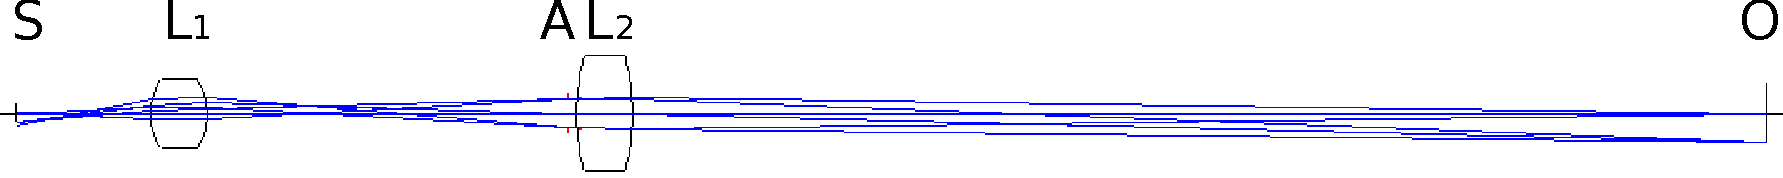
\includegraphics[width=1\columnwidth]{figures/lens_system_l2}
\caption{\label{fig:ls2_p}
WinLens plot of the simulation of the extended optical system with lens~2.
From left to right:
Sensor plane~S,
original mouse lens~L$_1$,
aperture A,
second lens~L$_2$ and
object plane~O.
}
\end{center}
\end{figure}

\begin{figure}[htbp]
\begin{center}
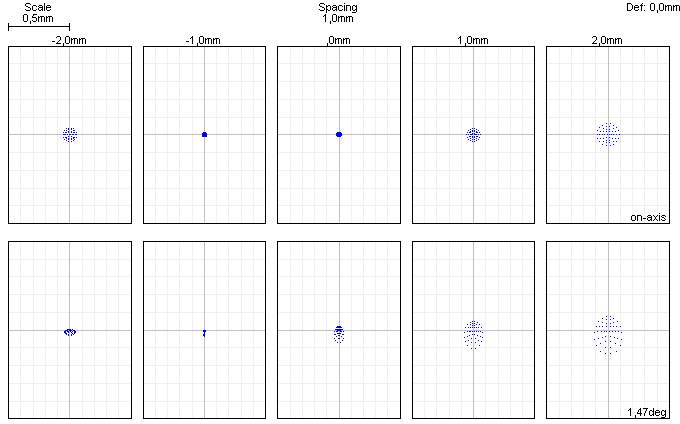
\includegraphics[width=1\columnwidth]{figures/spot_diagram_2lenses.png}
\caption{\label{fig:ls2_s}
WinLens plot of the spot diagram of the simulation of the extended optical system with lens~2, $\lambda = 842$\,nm.
The focusing of the spots hint to a relatively well modelled system.
}
\end{center}
\end{figure}

\subsubsection{Optical Path Calculations: Telecentric Setup}

Until now, the magnification of the system (And therefore the measured speed) is linear dependant on the object distance, which we wished to vary about $\pm 10$\,mm.
This would induce unacceptable errors from varying object distance.
To counter that, the distance-dependant magnification can be eliminated by a telecentric attachment.\\
To make a finite conjugate system like ours telecentric, a lens with the focal length of the object distance has to be placed in front of the objective, with its focal point set into the aperture of the objective~\cite{telec}.
The third lens is therefore placed at the position of the object of the 2-lens set-up, as seen in~\autoref{fig:sketch-optic-simple} in~\autoref{optics}.
As telecentric lens, an achromatic doublet with $f=50$\,mm is used.
This does not alter the magnification, and the sharpness remains in an acceptable range up to 30\,mm from the telecentric lens.
The choice of this lens type has been approved by WinLens simulation, see~\autoref{fig:ls3_p} and~\autoref{fig:ls3_s}.


\begin{figure}[htbp]
\begin{center}
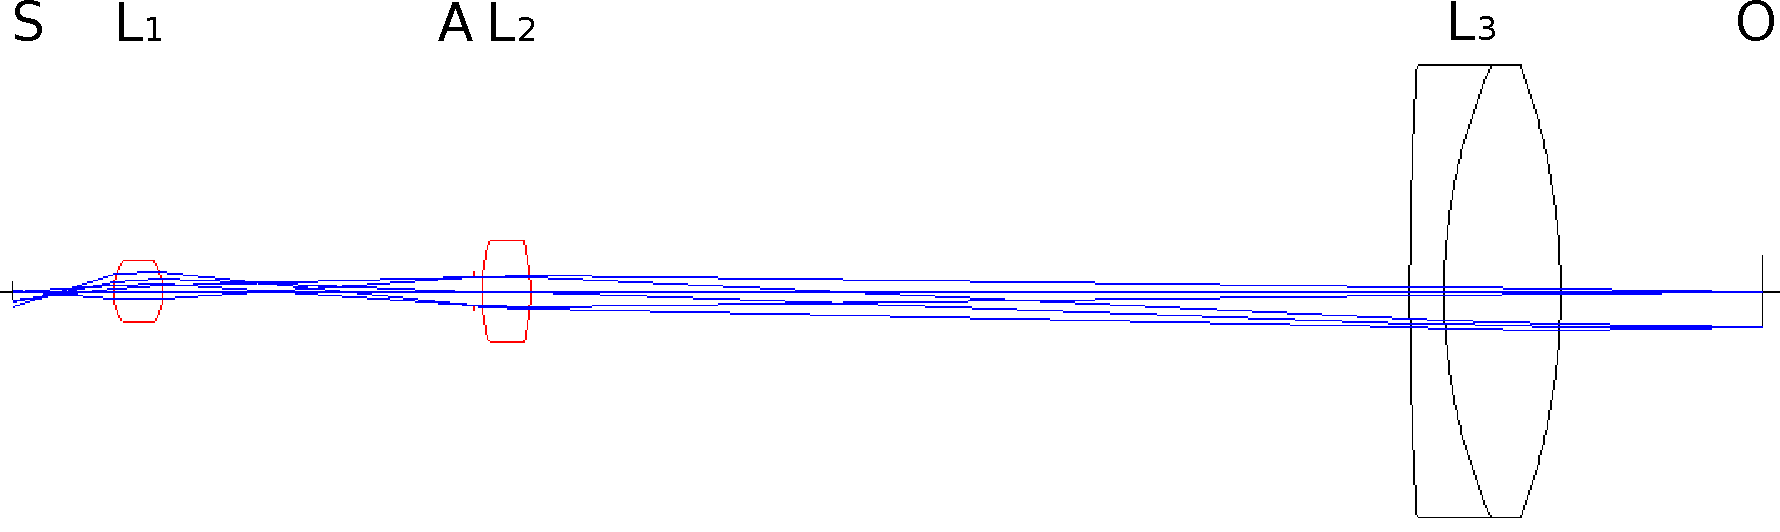
\includegraphics[width=1\columnwidth]{figures/lens_system_telecentric.pdf}
\caption{\label{fig:ls3_p}
WinLens plot of the telecentric system with all three lenses.
From left to right:
Sensor plane~S,
original mouse lens~L$_1$,
aperture A,
second lens~L$_2$,
third lens~L$_3$ and
object plane~O.
}
\end{center}
\end{figure}

\begin{figure}[htbp]
\begin{center}
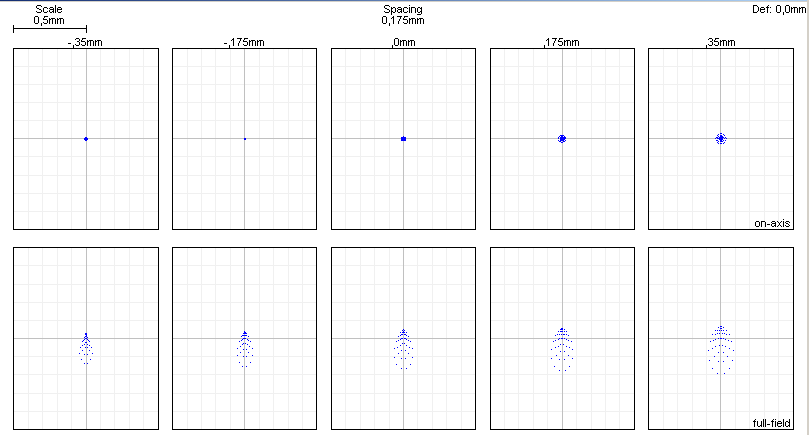
\includegraphics[width=1\columnwidth]{figures/spot_diagram_telecentric.png}
\caption{\label{fig:ls3_s}
WinLens plot of the spot diagram of the simulation of the complete optical system, $\lambda = 842$\,nm.
The focusing of the spots hint to a relatively well modelled system.
}
\end{center}
\end{figure}

\subsubsection{Sensor Mounting and Calibration}
\label{semo}

The PCB for the ADNS-6010 (as shown in~\autoref{fig:testplatine-board} in~\autoref{adns-pcb}) is mounted on a Micro-Bench carrier.
Its mount allows for calibration of the sensor in x- and y-position as well as the angle of the sensor to the optical axis of the Micro-Bench.
The PCB is mounted in an $21.5^\circ$-angle due to the angle of the optical axis on the ADNS-6010 (as shown in~\autoref{fig:o_setup_datasheet}).
The mount and the position of all calibration screws is shown in~\autoref{fig:sens-mount}.

\begin{figure}[htbp]
\begin{center}
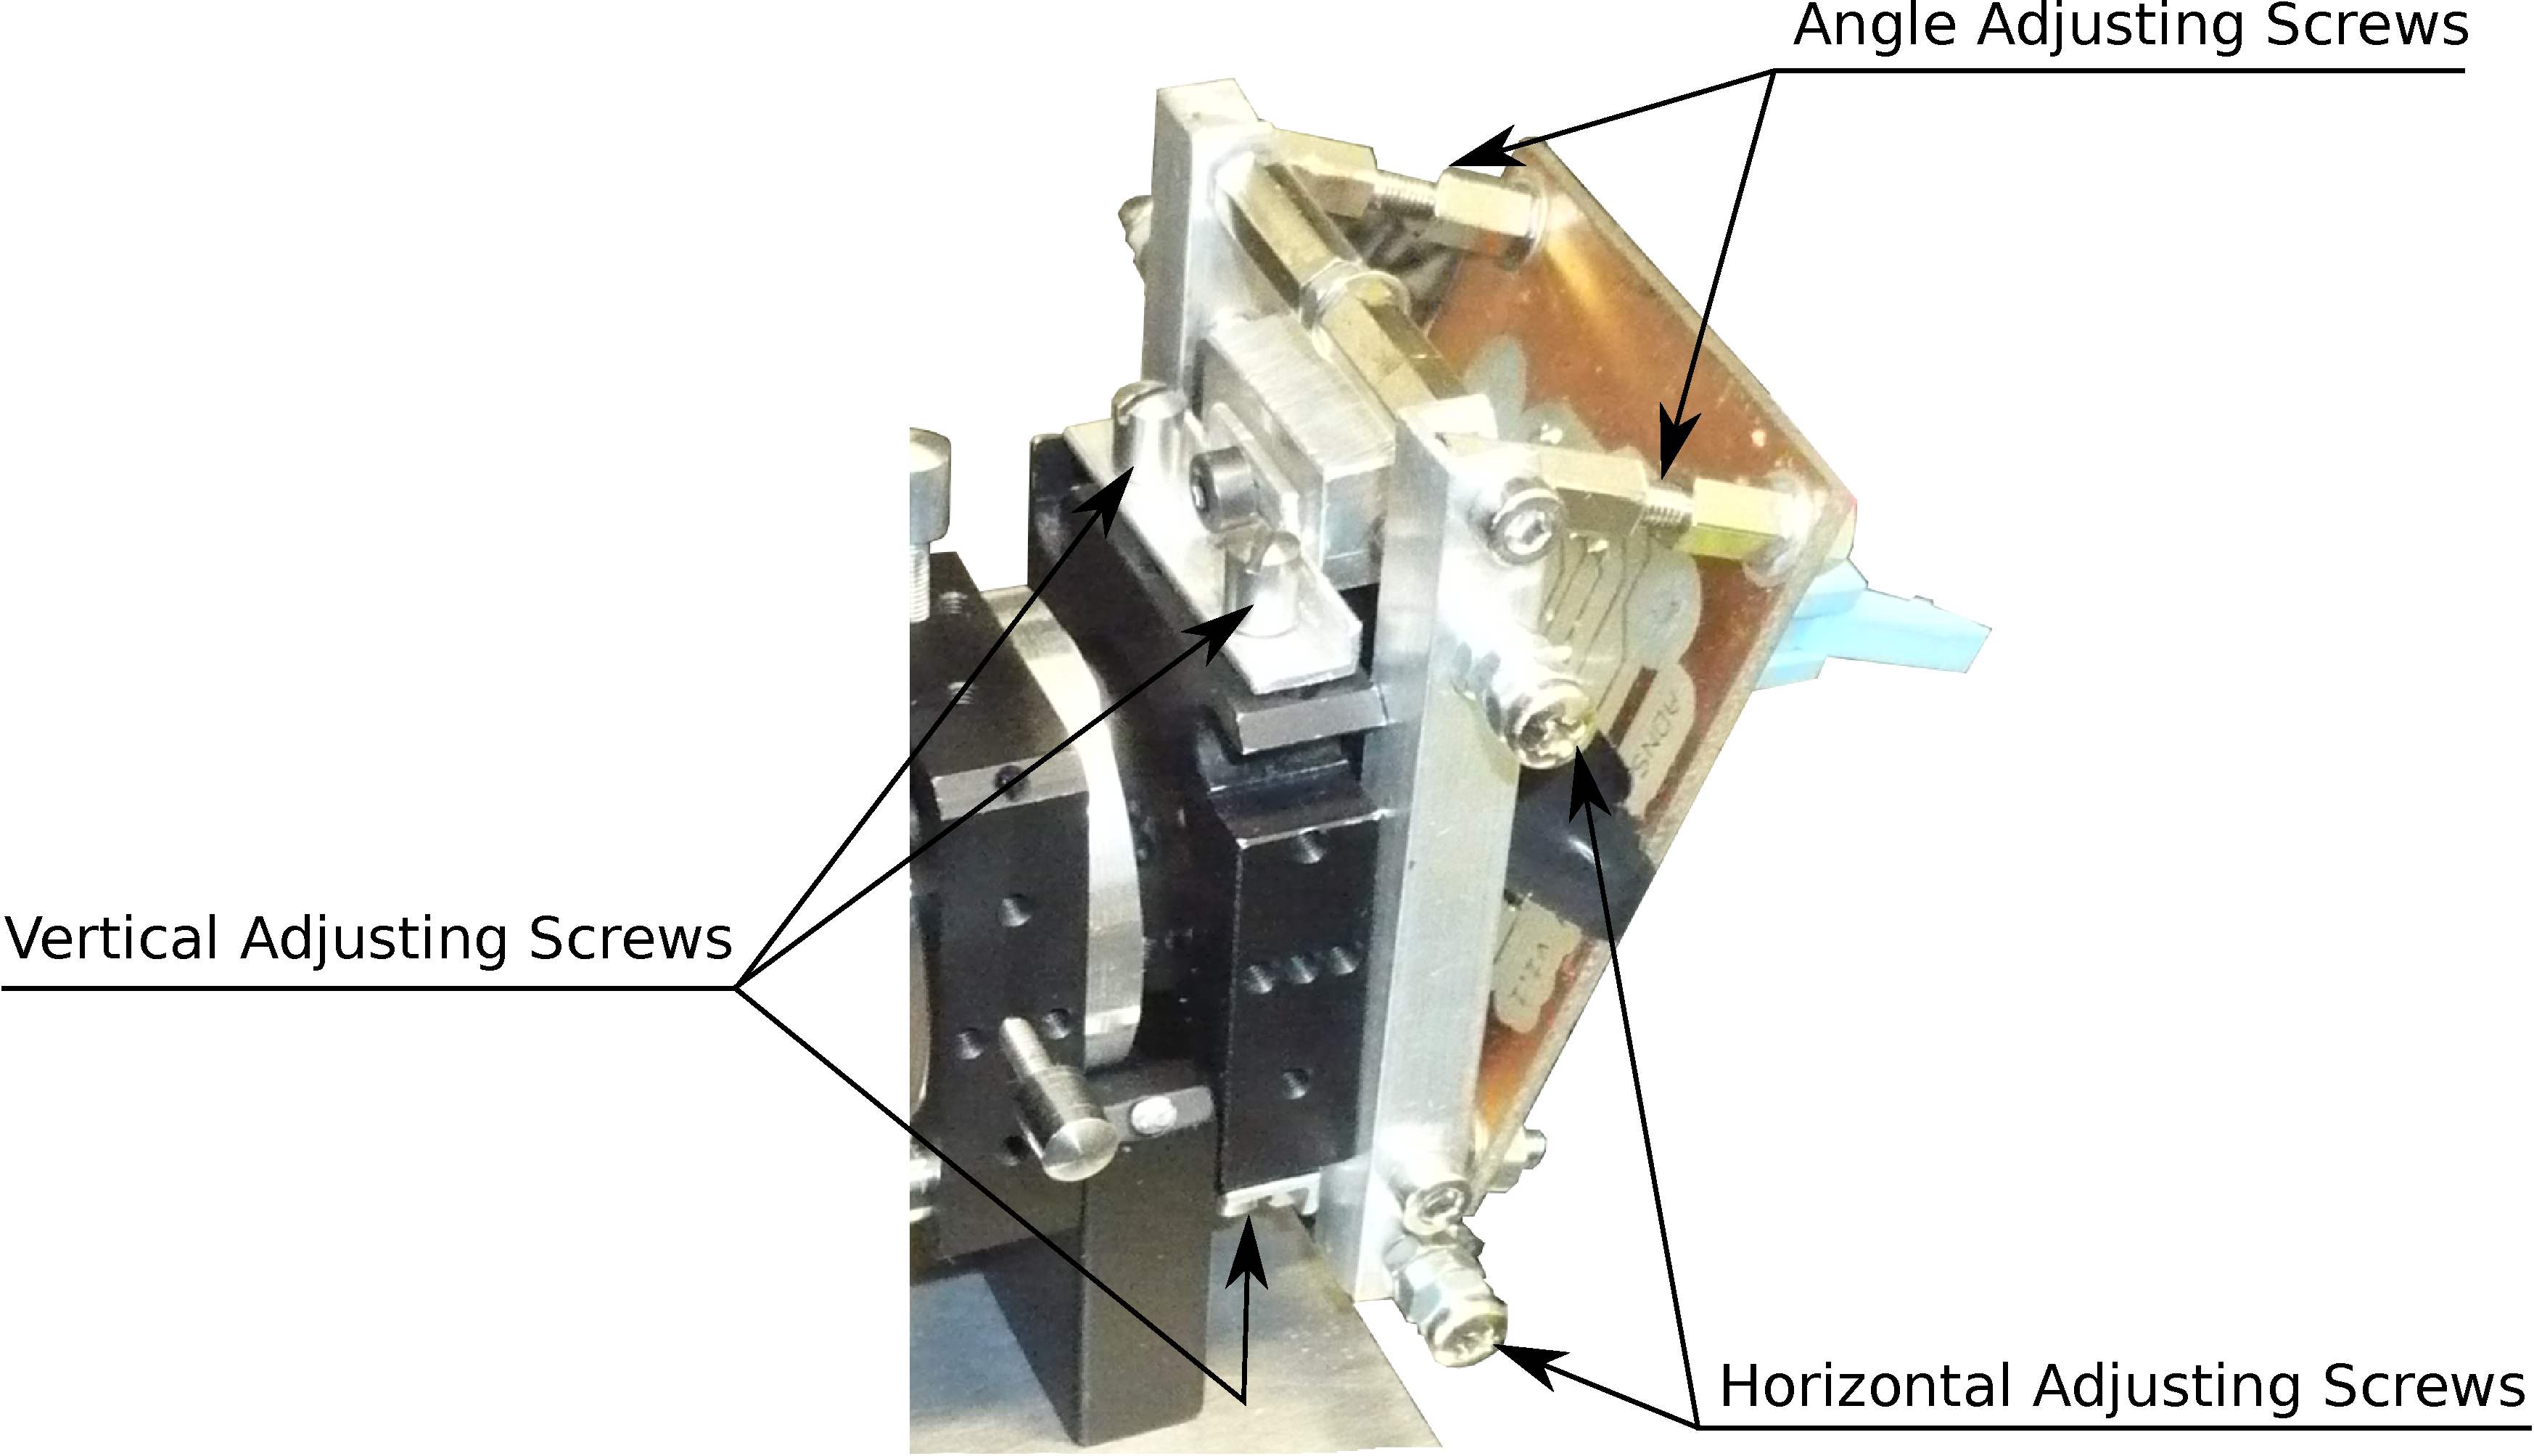
\includegraphics[width=1\columnwidth]{figures/sens-mount.pdf}
\caption{\label{fig:sens-mount}
The PCB with the ADNS-6010 with its mount on a Micro-Bench carrier on the end of the Micro-Bench.
It can be adjusted horizontal and vertical to the optical axis of the Micro-Bench.
There are two pairs of opposite adjusting screws for each direction, horizontal and vertical.
Its angle can be adjusted with the variable PCB-holding screws on top.
}
\end{center}
\end{figure}

For calibrating the sensor to the optical axis of the Micro-Bench, it is mounted on the micro-bench with an IR-laser that defined the optical axis.
The set-up for calibration is shown in~\autoref{fig:cal_setup}.
The 5\,mW-laser\footnote{750\,nm, Model FIXME} has to be dampened by a filter-array for safety of the sensor.
In front of the sensor is the magnification lens L$_2$, which allows for a more accurate calibration with its $5\times$-magnification factor.
The sensor is connected to the microcontroller, and the image of the sensor is read out and visualized on a computer screen (For details of this process see~\autoref{software}).
The sensor is calibrated to the optical axis by trying to move the laser speckle in the image to the centre by changing sensor position with the adjusting screws.
A sample image of the laser pointing to the sensor from the sensor's view can be seen in~\autoref{fig:image-laser}.

\begin{figure}[htbp]
\begin{center}
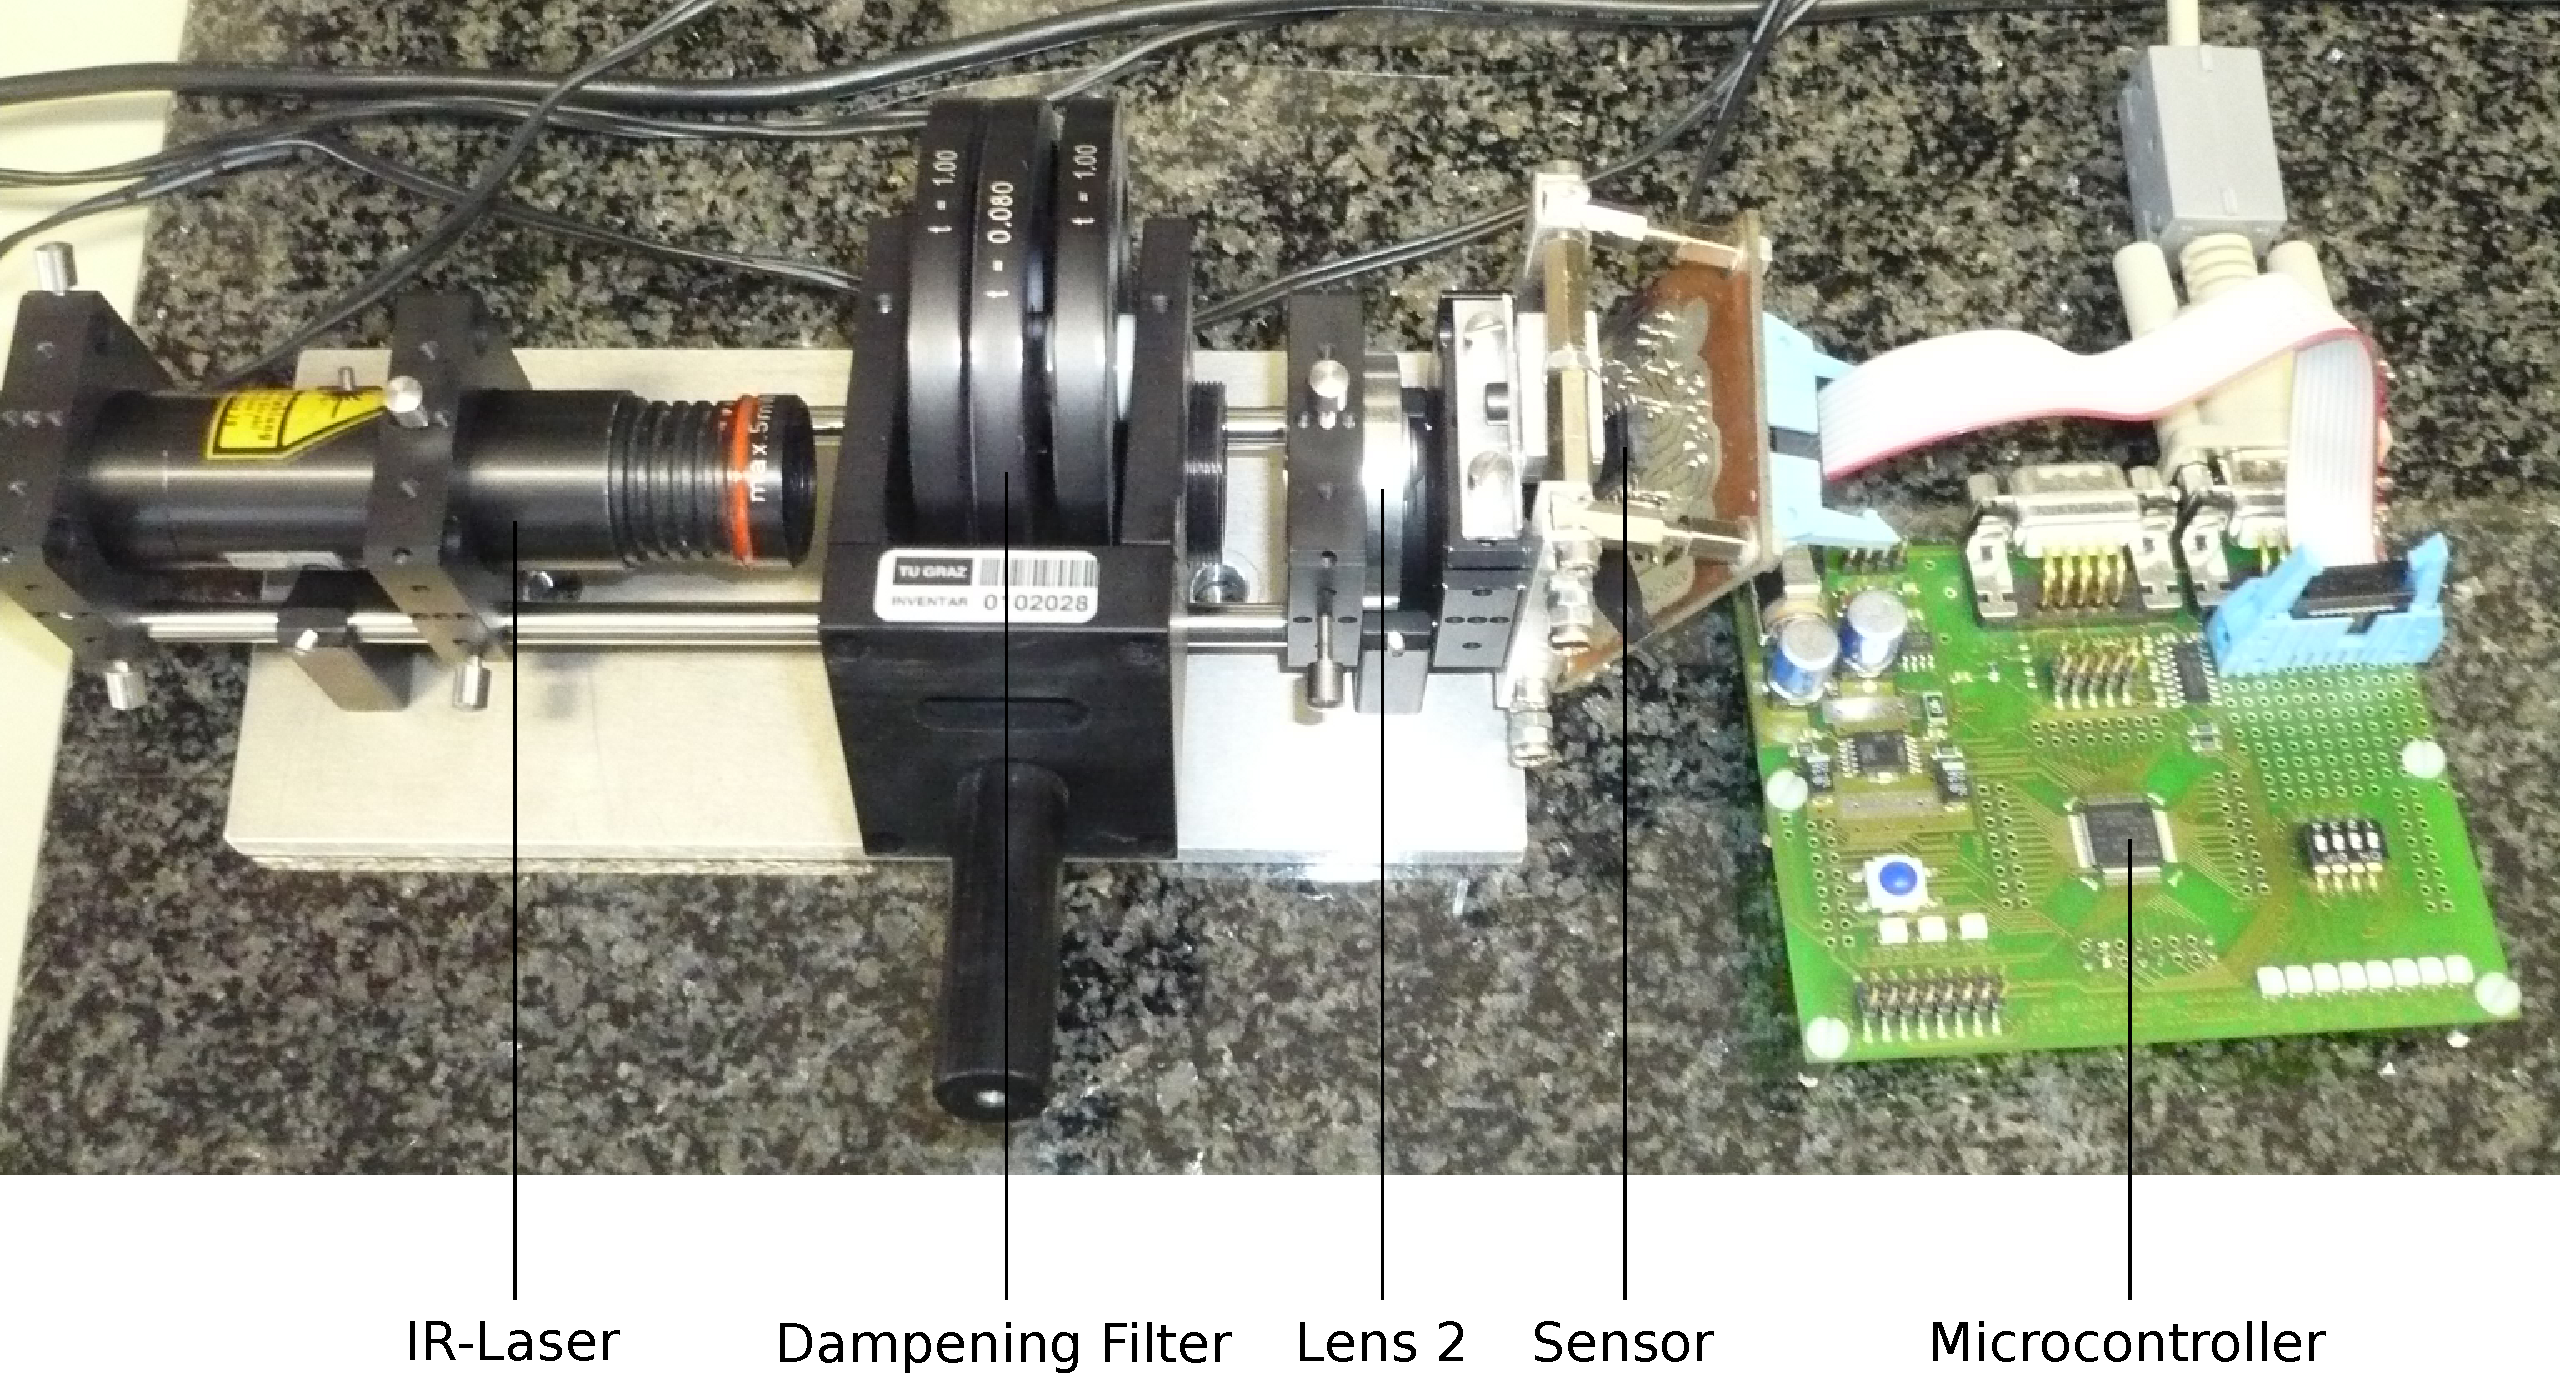
\includegraphics[width=1\columnwidth]{figures/cal_setup.pdf}
\caption{\label{fig:cal_setup}
Set-up for calibrating the sensor to the optical axis of the Micro-Bench.
From left to right:
IR-laser,
laser dampening filter,
magnification lens~2 in front of the sensor and the microcontroller for reading out the sensor image.
}
\end{center}
\end{figure}


\begin{figure}[htbp]
\begin{center}
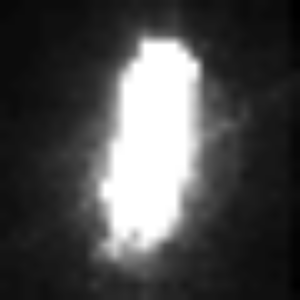
\includegraphics[width=0.4\columnwidth]{figures/sensor_image_laserspot.PNG}
\caption{\label{fig:image-laser}
Image of the laser speckle in the calibration process from the sensor's view.
$30\times30$\,px$^2$ resolution, 264\,$\muup$s shutter length.
}
\end{center}
\end{figure}

\subsubsection{Lens 2 and Aperture Mounting}
\label{l2m}

According to the calculations in~\autoref{opt:2l}, a lens\footnote{N-BK7 Bi-Convex Lens with IR-coating (LB1157-B)} with $f=10$\,mm was ordered from Thorlabs\footnote{\url{http://www.thorlabs.de} as on 08/01/2011}, along with an adapter\footnote{Adapter for \diameter\,6\,mm Optics (LMRA-6)} to 12.7\,mm ($\sfrac{1}{2}''$) diameter.
Its small diameter (6\,mm or 12.7\,mm with adapter) is not compatible with any Micro-Bench carrier available.
So a mount for both L$_2$ and the aperture is designed, which could be fixed in a 35\,mm-Micro-Bench carrier.\\
The mount is turned out of aluminium with a cavity for the 12.7\,mm~lens adapter and mounting holes for the aperture.
It has four M3 mounting holes, two for the lens holder and two for the aperture.
The lens holder is held down by two bigger washers, the aperture mounted through its holes with distance washers.
The complete assembly is shown in~\autoref{fig:l2mount}.
The UniGraphics drawing of the mount is available in the AFS\footnote{\url{/afs/robocup.tugraz.at/mechanics/01_Krikkit3G/06_Odometriesensoren/CAD/Versuchsaufbau/Linsenhalterunghalterung/} as on 08/01/2011}.

\begin{figure}[htbp]
\begin{center}
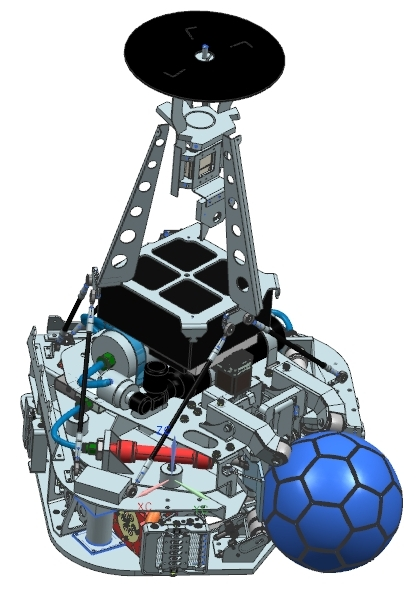
\includegraphics[width=0.4\columnwidth]{figures/Krikkit3G.jpg}
\caption{\label{fig:l2mount}
FIXME take image from lens mount!
Lens mount for L$_2$ and the aperture.
The lens in its adapter is held down by two washers,
the aperture is mounted with distance washers as close as possible to the lens.
}
\end{center}
\end{figure}

For the experiments, a set of apertures with different diameters are made.
They are made of copper-coated epoxy, normally used for PCBs.
The apertures are a simple sheet of epoxy the size $10\times40$\,mm$^2$ with the aperture in the middle and two mounting holes matching for the lens~2 mount outside.
They are manufactured on the circuit board plotter of the \EMT. 
The EAGLE files for the aperture plates are available in the AFS\footnote{\url{/afs/robocup.tugraz.at/projects/2010_improved-odometry/platinen/Blenden} as on 08/01/2011}.
Eight different aperture plates with aperture diameters 0.7, 0.8, 0.9, 1.0, 1.2, 1.5, 1.8 and 2.1\,mm are manufactured.
The apertures must be mounted with the copper side facing the lens on the lens mount to sit as close as possible to the lens surface.

\subsubsection{Illumination}

The original illumination for the laser mouse consists in a VCSEL laser diode with a wavelength of 842\,nm.
With the magnification system, we have a much greater target area to illuminate, for which the original VCSEL is too weak.
The goal is to find a proper illumination for a target area of $5\times5$\,mm$^2$.
It must be bright enough on every test surface (see \autoref{}) %FIXXME chapter requirements
to allow the automatic shutter control of the sensor minimize the shutter for the maximum frame-rate. 
Other requirements are the available space on the robot for a sensor, and the power consumption. 
The illumination must fit besides the optical ray path inside the space constraints of the $60\times60$\,mm$^2$ cross-section.
The power supply are either 24 or 6\,V, and the cooling possibilities are limited by the space constraints.\\
The frequency of the illumination must be in the range of the responsivity of the ADNS-6010, see~\autoref{fig:resp}.
A monochromatic light source would find favour, as this would lead to higher contrast.

\begin{figure}[htbp]
\begin{center}
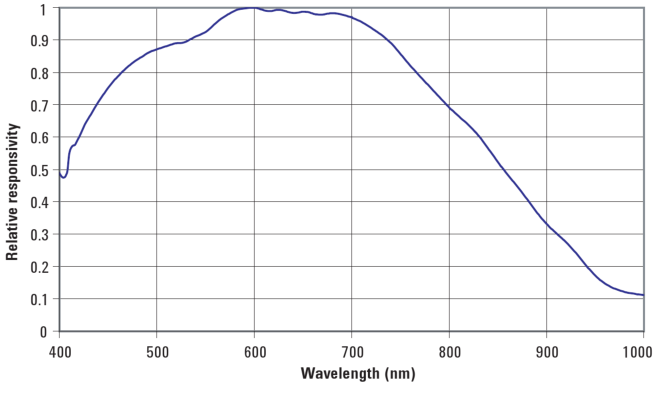
\includegraphics[width=0.6\columnwidth]{figures/responsivity}
\caption{\label{fig:resp}
Relative responsivity for the ADNS-6010 laser mouse sensor from the data sheet~\cite{adns}.
}
\end{center}
\end{figure}

Finding proper illumination is a difficult task, as every tested surface reacts differently on each type of illumination.
The illuminant tested are a 1\,kW studio spotlight, the laser used for calibrating and different types of high-power LEDs.
Every illuminant is tested on a white sheet of paper for reference, and then on the three different carpets.
For the experiments it is required for the illumination to achieve the maximum frame-rate of 7080\,Hz (shutter below 18\,$\muup$s) on all test surfaces accomplished by an acceptable surface quality (feature count around 100).
The shutter/frame-rate and surface quality were read out via the PyQt-application described in~\autoref{software}.\\
The studio spotlight could not be focused enough on the $5\times5$\,mm$^2$ spot to achieve the luminous density needed to achieve the needed frame-rate on any of the test surfaces.
Example screen-shots of the studio spotlight illuminating the test surfaces can be seen in~\autoref{fig:ill-spotlight} for every test surface.
The studio spotlight would need more focusing optics to reach the luminous density needed, and even using a smaller version would not fit on the robot, so smaller approaches follow next.\\
For the laser used for calibration, due to its power and beam size being similar to the original VCSEL, it was too weak to be used.\\
The best power/size rating can be achieved with LEDs.
The brightest LEDs found were from \href{http://www.led1.de}{LED1.de}.
Two types of LEDs were chosen for comparison, ultra-bright white LEDs and infra-red LEDs.
Their specifications can be seen in~\autoref{table:leds}.

\begin{figure}[htbp]
  \begin{center}
    \mbox{
      \subfigure[White sheet of paper]{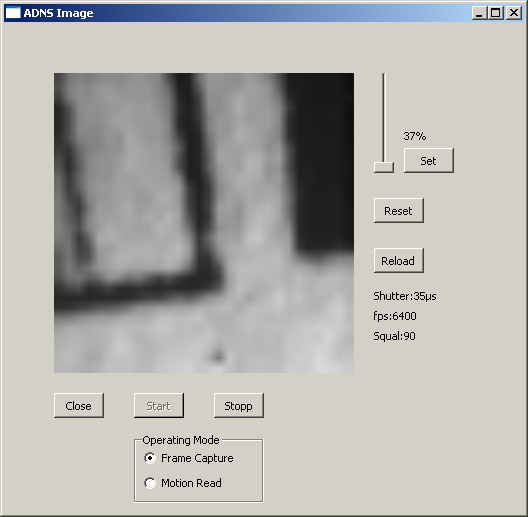
\includegraphics[width=0.48\textwidth]{figures/beleuchtung-papier-scheinwerfer-blende10.PNG}} \hfill
      \subfigure[Carpet 1]{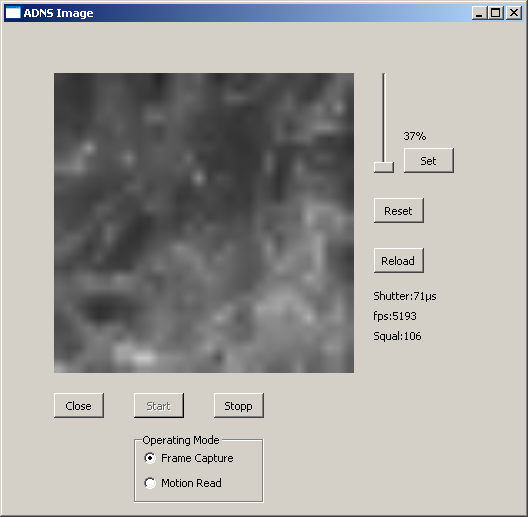
\includegraphics[width=0.48\textwidth]{figures/beleuchtung-teppich1-scheinwerfer-blende10.PNG}}
      }
    \mbox{
      \subfigure[Carpet 2]{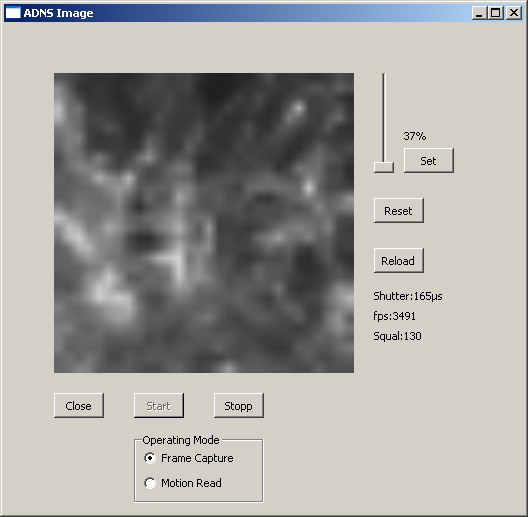
\includegraphics[width=0.48\textwidth]{figures/beleuchtung-teppich2-scheinwerfer-blende10.PNG}} \hfill
      \subfigure[Carpet 3]{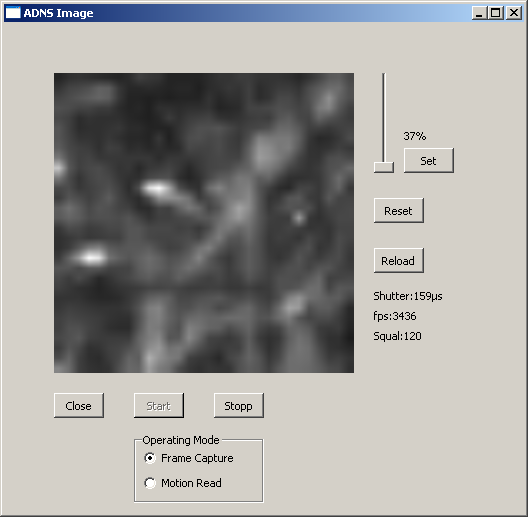
\includegraphics[width=0.48\textwidth]{figures/beleuchtung-teppich3-scheinwerfer-blende10.PNG}}
      }
    \caption{Screen shots of the four target surfaces (a--d) with illumination by the studio spotlight.
The distance of the spotlight to the surface was 17\,cm.
An aperture of 1.0\,mm was used.
The surface quality (Squal) of all samples is sufficient, but the needed frame-rate (fps) of 7080\,Hz is not reached anywhere.
The software used is described in~\autoref{software}.}
    \label{fig:ill-spotlight}
  \end{center}
\end{figure}

\begin{table}[htbp]
  \begin{minipage}{0.45\textwidth}
    \centering
    \begin{tabular}{r|l}
       %\hline
%       Property & Value \\
       Name  & Nichia NSPW500GS-K1     \\
       \hline
       Art.\ \# & \href{http://www.led1.de/shop/product_info.php?pName=nichia-nspw500gsk1-led-5mm-white-44000mcd-10-pcs-p-1161&cName=led-5mm-ultra-bright-white-44000mcd-nichia-c-3_276&xploidID=4a06ee48002afb920a3a4663e80b324d}{54400101} \\
       Case & 5\,mm waterclear     \\
       Viewing Angle  & 15$^\circ$     \\
       Power & 3.2\,V     \\
       Current & 20\,mA typ., 30\,mA max.     \\
       Brightness & 44\,000\,mcd     \\
       Price & 9.99 \euro\ (10 pcs.)     \\
       Chromaticity \\
       Coordinates x/y & 0.31/0.32     \\
    \end{tabular}
  \end{minipage}\hfill
  \begin{minipage}{0.45\textwidth}
    \centering
    \begin{tabular}{r|l}
%      Property & Value     \\
       Name  & LED 5\,mm infrared     \\
      \hline
       Art.\ \# & \href{http://www.led1.de/shop/product_info.php?=&pName=led-5mm-infrared-850nm-120mw-10-pcs-p-1349&cName=led-5mm-ultra-bright-infrared-850nm-120mw-c-3_277&xploidID=4a06ee48002afb920a3a4663e80b324d}{50885002} \\
       Case & 5\,mm waterclear     \\
       Viewing Angle  & 15$^\circ$     \\
       Power & 1.5\,V     \\
       Current & 50\,mA     \\
       Intensity & 120\,mW     \\
       Price & 7.99 \euro\ (10 pcs.)     \\
       Wave Length & 850\,nm (infrared)     \\
       &
    \end{tabular}
  \end{minipage}
  \caption{Technical data of both LED types evaluated.
  LEDs ordered from \href{http://www.led1.de}{LED1.de}, prices from 30/10/2010.}
  \label{table:leds}
\end{table}

From each type of LEDs, 20 pieces were ordered.
Any single LED of these provides still not enough luminous density, so an array of these LEDs is used.
They must be mounted as close as possible to the target surface.
The only possible mounting place on the micro-bench is between the second and the third lens, see~\autoref{fig:illm}.
They are mounted in a ring around the optical rays, and illuminate the surface through the third lens.
Therefore, a small PCB is designed\footnote{EAGLE files are available in the AFS:\url{/afs/robocup.tugraz.at/projects/2010_improved-odometry/platinen/LED_ring_v2} as on 15/01/2011} with nine LEDs in a circular array, and an opening in the centre for the optical beam~(\autoref{fig:illupcb}).
It is designed to fit on the micro-bench, and is then mounted on a micro-bench carrier.

\begin{figure}[htbp]
\begin{center}
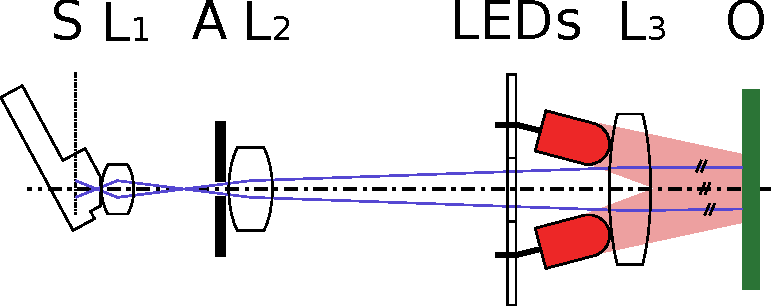
\includegraphics[width=0.8\columnwidth]{figures/sketch-optic.pdf}
\caption{\label{fig:illm}
Complete optical system with illumination.
The LEDs are placed on a PCB in a circle around the optical ray path, and illuminate the object surface~(O) through the third lens~L$_3$.
The effect of the third lens on the illumination rays is negligible.
}
\end{center}
\end{figure}

\begin{figure}[htbp]
  \centering
  \subfigure[Illumination PCB circuit]{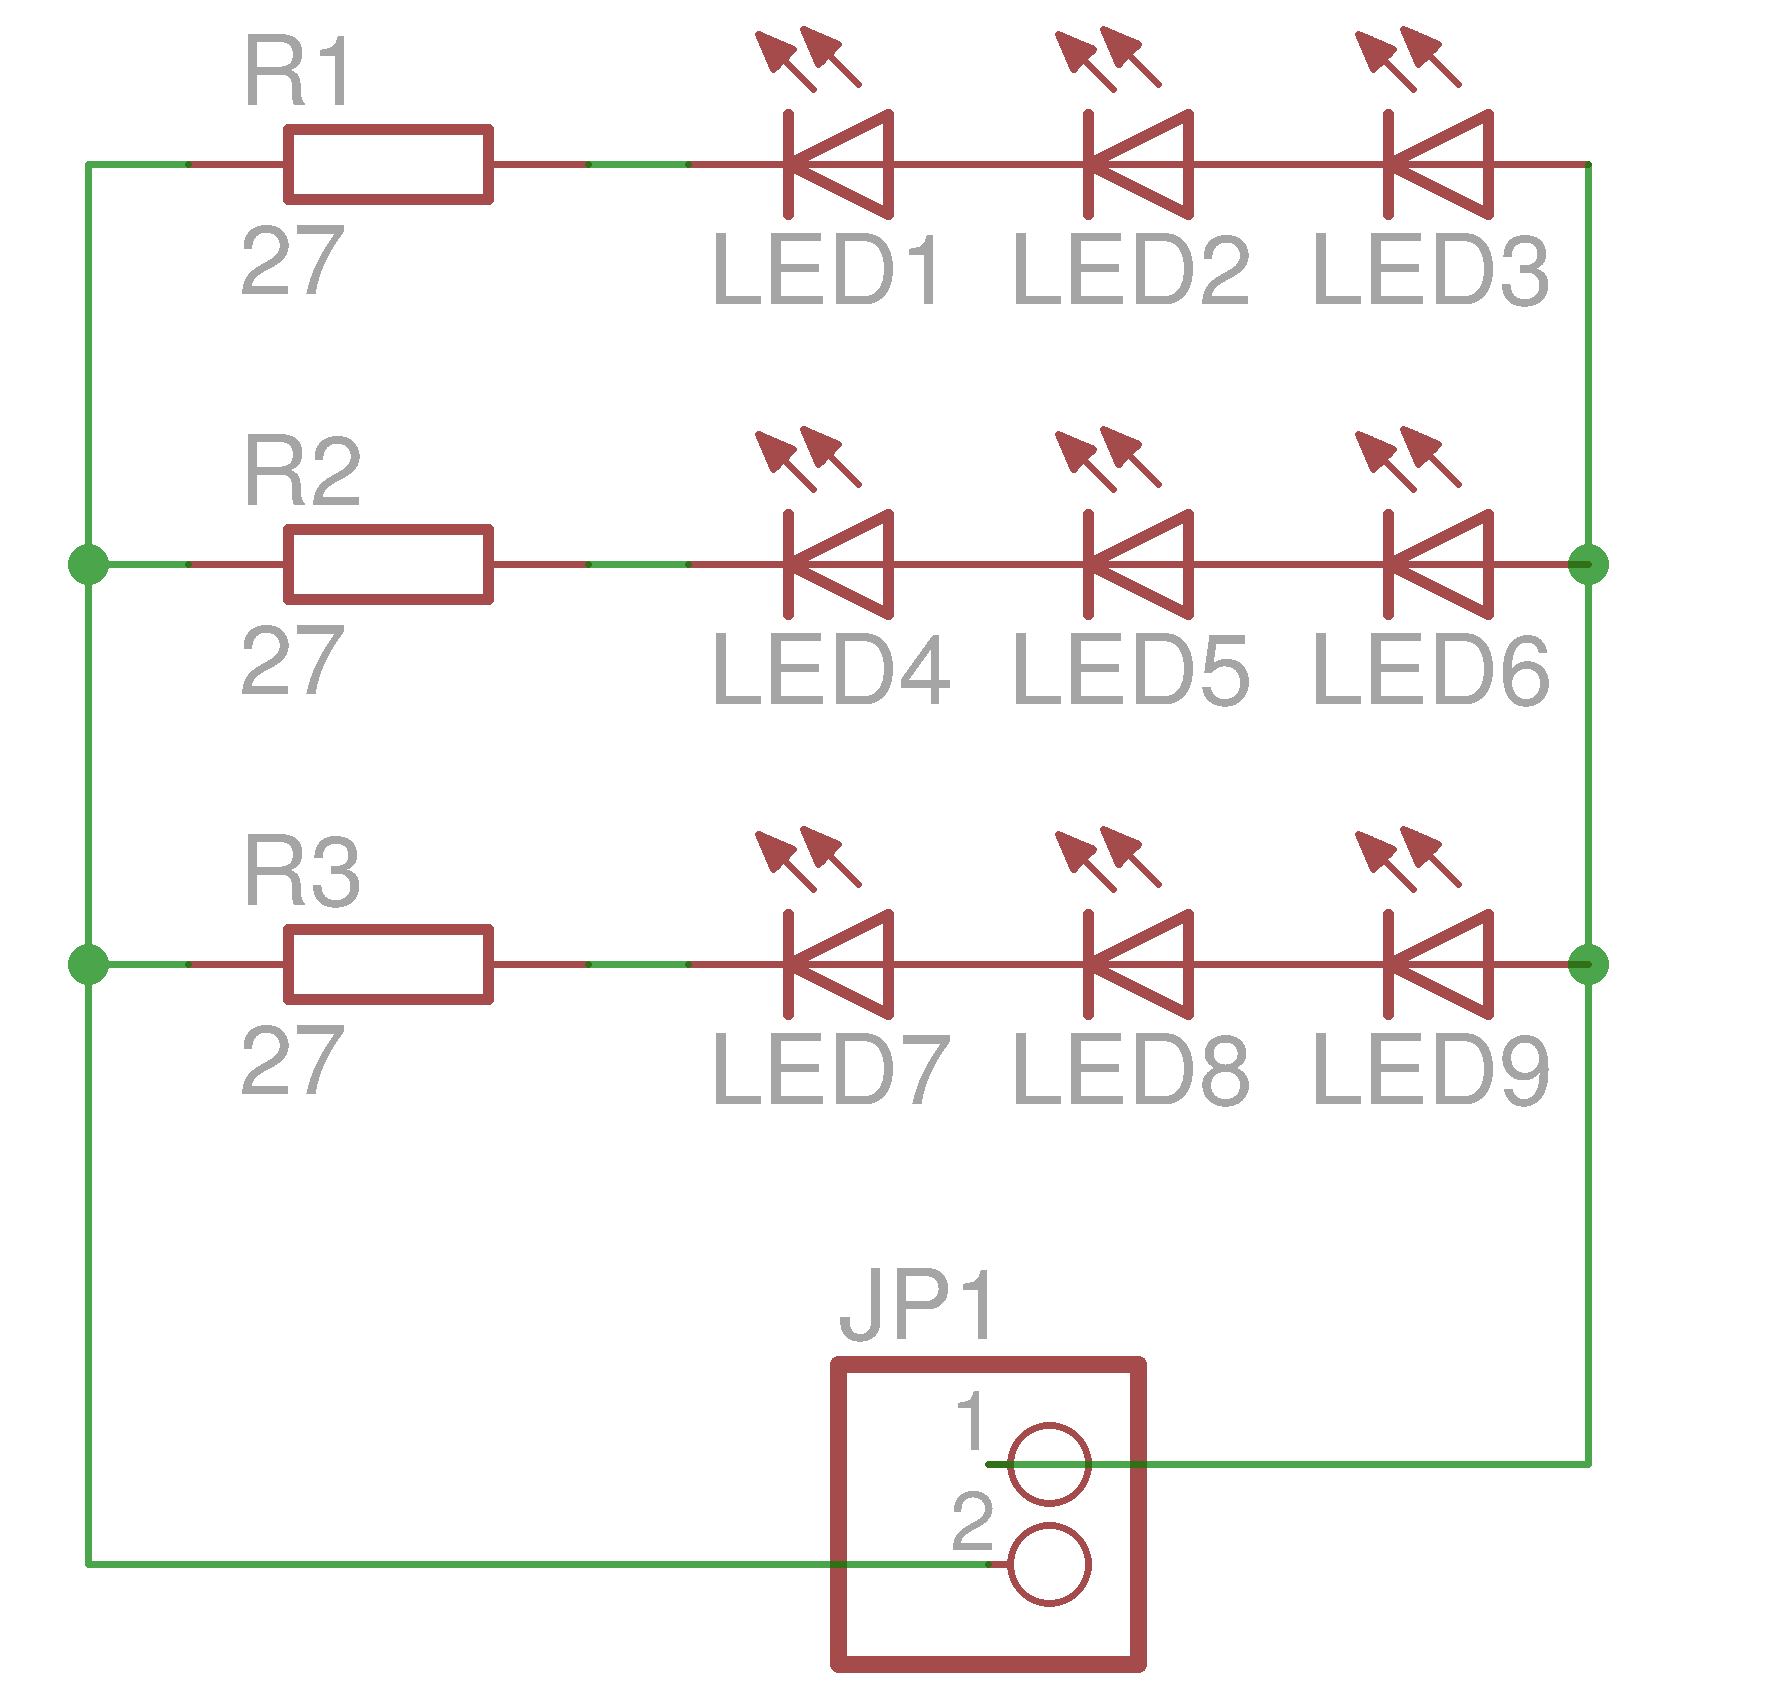
\includegraphics[width=0.5\textwidth]{figures/LED-layout.png}} \hfill
    \subfigure[Illumination PCB board layout. Sketch not to scale.]{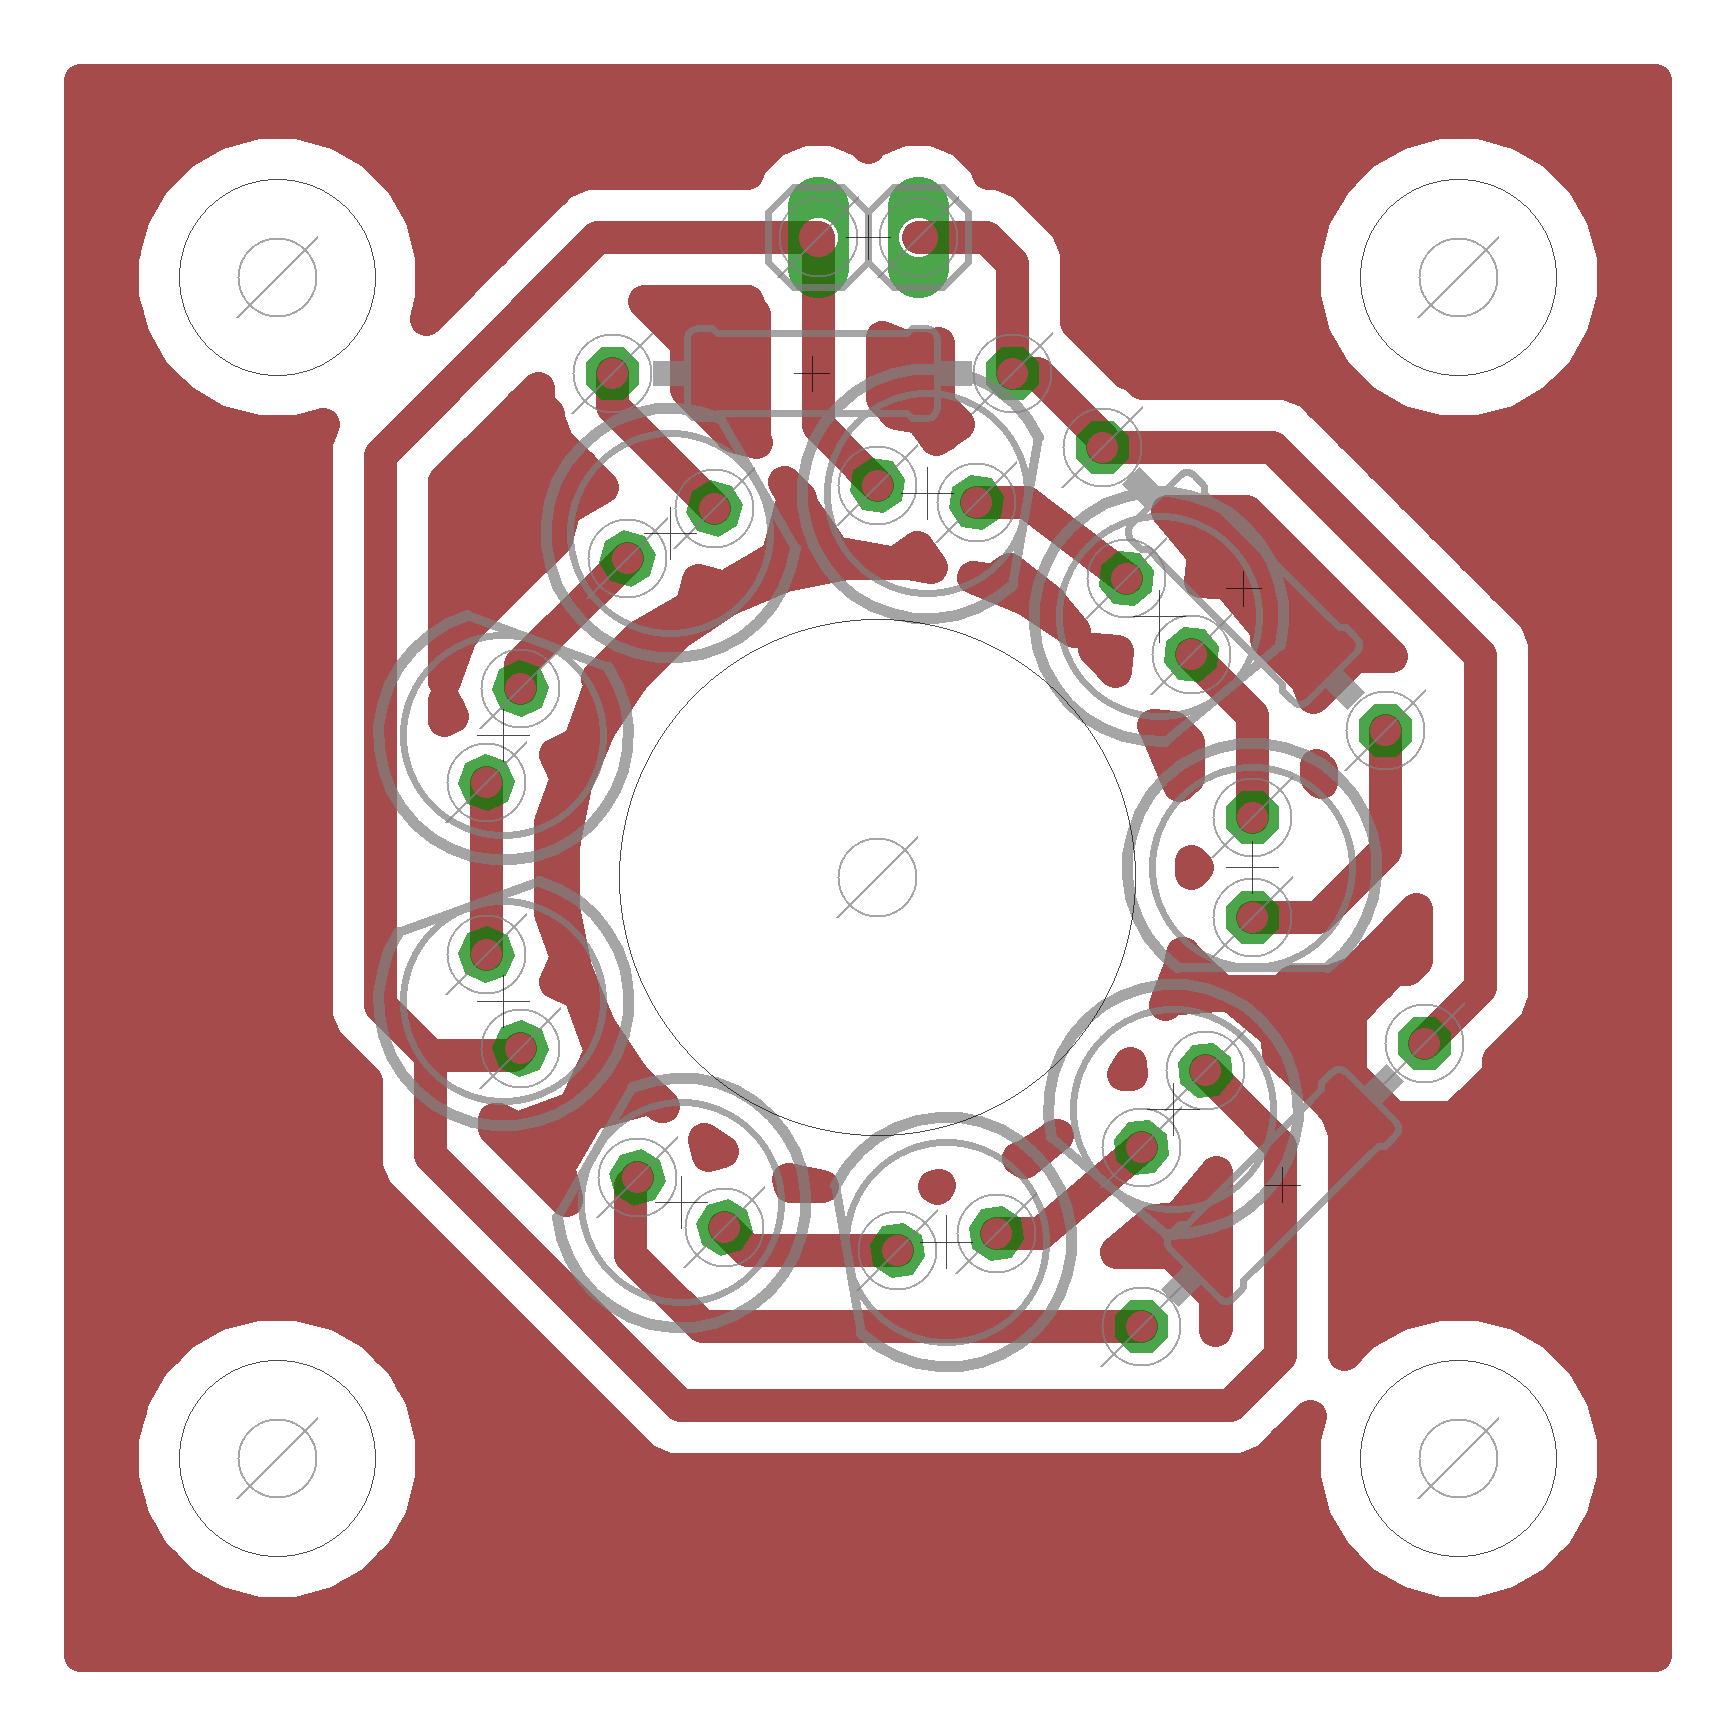
\includegraphics[width=0.40\textwidth]{figures/LED-board.png}}
  
  \caption{Illumination PCB circuit and layout. 
  The PCB is designed to be mounted on the micro-bench with the corner-holes and measures $40\times40$\,mm$^2$. 
  Nine LEDs are arranged around the centre hole for the optical rays.
  To reduce the overall voltage needed, they are arranged in three parallel lines with three LEDs and a series resistor each.
  The power supply is to be connected on a simple 2-pin header on top.}
  \label{fig:illupcb}
\end{figure}

From the PCB, four pieces were manufactured for testing.
They are populated with either white or infra-red LEDs.
Power must be supplied by an external power supply unit.
Both LED types are to be powered with a constant current source.
According to~\autoref{table:leds}, for the PCBs with white LEDs for which a maximum current of 30\,mA is allowed, 90\,mA for the three lines are used, and 150\,mA for the infra-red LEDs.
With the serial resistor, this leads to a needed voltage of $\approx\unit[22]{V}$ for the white LEDs and $\approx\unit[10]{V}$ for the infra-red LEDs.
It would be possible to achieve more luminosity with the LEDs operating at higher currents in PWM mode~(using the PWM signal for the original VCSEL from the sensor), however the constant current luminosity was enough for the experiments.\\
The nine LEDs need to be aligned to point exactly to the target centre for the maximum effect.
Every LED on the PCB is calibrated separately to point to the centre.
For the white LEDs, this can be seen in~\autoref{fig:led-cal}.
The infra-red LEDs are calibrated via the streamed video from the sensor, as their light (850\,nm) is invisible to the human eye.\\
A note on the cooling of the LEDs: They got very warm, but this was no problem in the open testbed.
When tightly packed inside the robot, an appropriate cooling strategy must be considered.

\begin{figure}[htbp]
\begin{center}
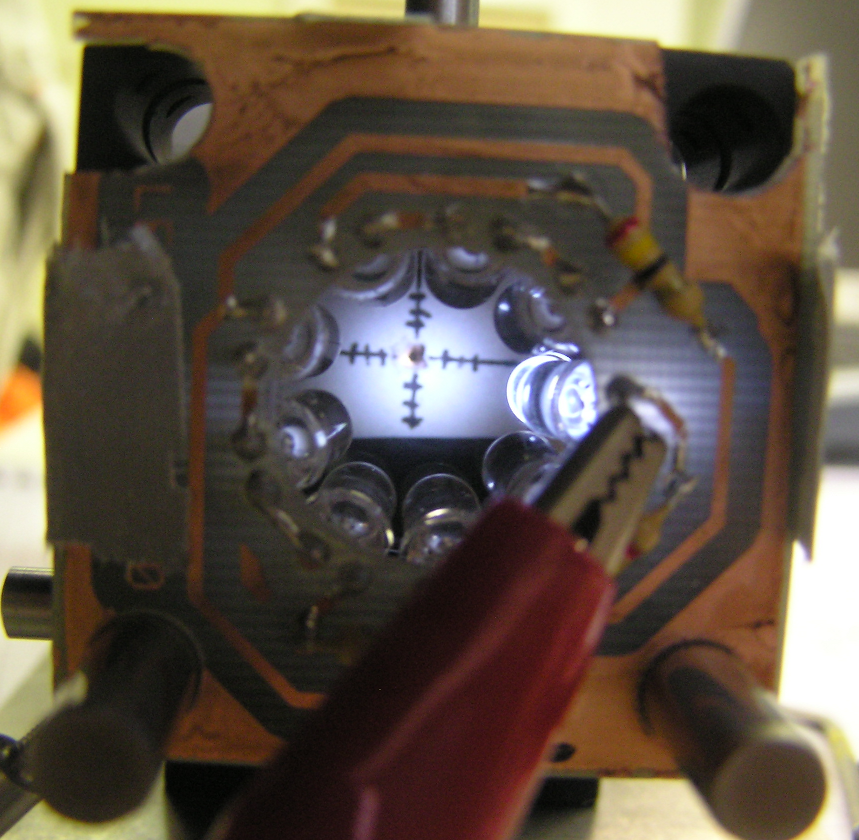
\includegraphics[width=0.5\textwidth]{figures/led-centre-cal.png}
\caption{\label{fig:led-cal}
Calibration of the LEDs to point to the centre for maximum effect.
The angle of every LED on the PCB is calibrated separately to point to the marked centre.
}
\end{center}
\end{figure}


When comparing the white and infra-red LEDs, the infra-red LEDs perform slightly better, so the experiments are done with infra-red illumination.


\subsection{Software}
\label{software}

The software required for controlling the sensor is split into two parts: 
The low-level interface for directly communicating with the ADNS-6010 laser mouse sensor is implemented in the microcontroller software written in~C.
The software on the microcontroller is again commanded from the user interface running on the~PC written in Python and~Qt (PyQt).\\
The user interface displays the images read from the sensor, or logs motion data into text files.
These text files are analysed and the results are plotted with octave.

\subsubsection{Microcontroller-Software}

The microcontroller software is written in~C and developed with the Keil\footnote{Keil uVision3 V3.30a \copyright~Keil Software Inc.\ downloadable from: \url{http://www.keil.com}}~IDE. % FIXME footnote already in chapter
The Keil IDE produces hex files (*.H86), which are flashed over the serial port (RS-232) to the microcontroller development board.
For the flashing process, see the board manual~\cite{xc}.
It is important to use a high quality serial cable to avoid bit-errors on the flashing process.
The full source code of the software and the hex-binary is available in a git repository\footnote{\url{git://marvin.robocup.tugraz.at/git/uc_impodo_testbed.git} as on 15/01/2011}.

The  software on the microcontroller should fulfil the following functions:
Catch the firmware in stage~1
and in stage~2 flash the ADNS-6010 with the new firmware, 
read out images and motion data.\\
The microcontroller is connected to the PC via RS-232.
For communication via a terminal emulator from the PC, an interactive console has been implemented based on the motion controller code~\cite{krammer07}.


For the firmware catch, the syncronous serial interface~(SSC0) in slave mode is used together with an analogue input, where it waits for the reset signal from the original microcontroller.
The firmware is stored in the internal RAM of the microcontroller and can be output after the catch in human readable form on the terminal.
Due to the available RAM in the XC164-CM being smaller than the firmware size, the catch has to be split up.
It must be repeated with an offset given for four times, until the complete 1936\,Byte of the firmware are available.
After the firmware is known, it is integrated into the microcontroller program as static array, and can be flashed to the ADNS-6010 any time at stage~2.
The listening on the communication between the original mouse microcontroller and the ADNS-6010 revealed other interesting data:
After the firmware is flashed, the self test on the ADNS-6010 is triggered and the CRC of the firmware is checked.
Then some configuration parameters are set for the ADNS-6010:
The strength of the laser diode is set to 80\,\%, and the laser shutter mode is disabled. 
At last the resolution is set to 800\,dpi before starting motion read.

For the image read of the sensor, the image can either be output as PGM image on the terminal, or as binary data for use by the GUI.
It is interesting that the firmware must not be loaded on the ADNS-6010 before an image can be read out.
This largely increases the possible frame-rate of the video.
The bottleneck in video streaming is the serial line from the microcontroller to the host computer.
Therefore the speed of the RS-232 interface is increased to 115.6\,kbit/s, more is not possible with Windows~XP.
With an image size of 900\,Byte, a maximum frame-rate of 5~frames per second can be achieved, which makes the optical calibration processes very comfortable.\\
In motion read mode, the motion values read from the ADNS-6010 are output continuously on the serial port.
Before motion read, the firmware must be loaded to the ADNS-6010.
Data from the reference speed sensor (see~\autoref{lb}) is acquired in a background thread, and the current reference speed is output in addition to mouse sensor speed for comparison.

\subsubsection{PyQt GUI}

The microcontroller can be controlled completely via a command-line interface from a terminal emulator on the serial line.
But for displaying live images from the sensor, a graphical user interface (GUI) is needed.
Therefore a small GUI is developed, that can display images from the sensor and save motion data in a more convenient way.
The GUI is written in the Python\footnote{\url{http://www.python.org/} as on 17/01/2011} scripting language, with a Qt\footnote{\url{http://qt.nokia.com/} as on 17/01/2011} graphical user interface (PyQt\footnote{\url{http://www.riverbankcomputing.co.uk/software/pyqt/intro} as on 17/01/2011}).
The PyQt environment is chosen because of its cross-platform ability and the simple ways of creating a GUI.
The complete program with installation instructions is available in a git repository\footnote{\url{git://marvin.robocup.tugraz.at/git/impodo_gui.git} as on 17/01/2011}.
On Python modules, \emph{PyQt4} and \emph{serial} are needed.
The program uses the first serial interface (ttyS0 on Unix or COM1 on Windows), this can be changed in the constructor of the \emph{OdoFrame}-class.
The program is written completely threaded, and has two operation modes: Frame Capture and Motion Read.\\
The common controls and indicators for both modes are explained in~\autoref{fig:gui-common}.
It is possible to set the laser strength, load the firmware or reset the ADNS-6010 independent from operating mode.
After reset, the firmware must be loaded again if needed.

\begin{figure}[htbp]
\begin{center}
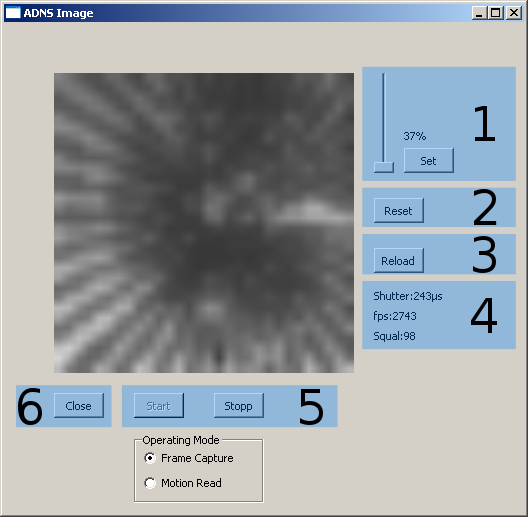
\includegraphics[width=0.8\textwidth]{figures/gui-common.png}
\caption{\label{fig:gui-common}
Screen-shot of the GUI with common controls and indicators.
On the right side controls with direct reference to the ADNS-6010:
Setting for the integrated laser driver with a range slider, where laser strength can be chosen between 37\% and 100\%. The setting is applied with the ``Set''-Button~(1).
The reset line for the ADNS-6010 is toggled with the ``Reset''-Button~(2).
The firmware of the ADNS-6010 can be reloaded with the ``Reload''-Button~(3).
Indicators for current Shutter, frame-rate (fps) and surface quality (Squal) in count of features~(4).
Beginning of frame capture or motion read is controlled with Start/Stop - Buttons~(5).
The ``Close''-Button terminates the program~(6).
}
\end{center}
\end{figure}

In frame capture mode, live images from the ADNS-6010 are displayed as a video with 5~frames per second.
After pressing the ``Start''-Button, a frame is captured, and after the ADNS-6010 is reset, the next frame is read.
This continues in a loop until the ``Stop''-Button is triggered.
It is not necessary to load the firmware before the frame capture, but it will be loaded before every frame if it was loaded from the beginning.
The display of the current shutter, frame-rate and surface quality is updated with each image.\\
In motion read mode, the display changes to a tabular view, where the current and accumulated motion data are displayed.
This view and the description of the entries is shown in~\autoref{fig:gui-motion}.
The firmware must be loaded before motion read can be started.
After pressing the ``Start''-Button, the motion read from the ADNS-6010 is started, and additionally to being displayed, all received data is written to a log-file.
Data is written in comma-separated value format, which is intended to be used as input for the octave analysis scripts described subsequently.

\begin{figure}[htbp]
\begin{center}
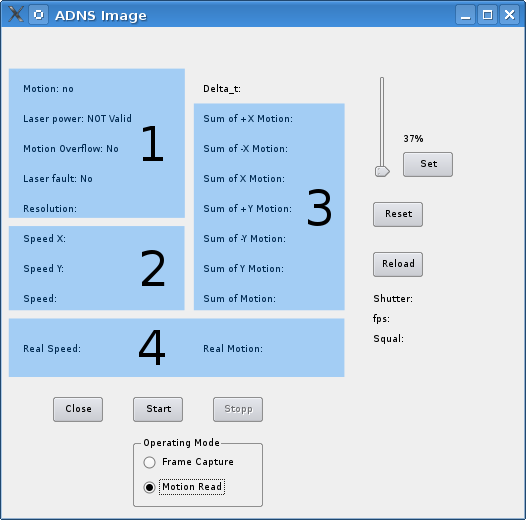
\includegraphics[width=0.8\textwidth]{figures/gui-motion-wtags.png}
\caption{\label{fig:gui-motion}
Screen-shot of the GUI in motion read mode.
Section~1 displays some status details of the ADNS-6010.
Section~2 shows the current speed calculated from the motion readings.
Section~3 shows the distance covered from the beginning of the motion read by accumulating every dimension.
Section~4 shows the speed and accumulated distance from the reference sensor connected to the microcontroller.
}
\end{center}
\end{figure}


\subsubsection{Octave Analysis Scripts}
\label{octave}

Mathematical data analysis is done in the GNU~Octave\footnote{\url{http://www.gnu.org/software/octave/} as on 20/01/2011} language, similar to Matlab.
The scripts process the csv-files produced with the GUI in motion-read mode.
They are available in the same git-repository\footnote{\url{git://marvin.robocup.tugraz.at/git/impodo_gui.git} as on 17/01/2011} as the GUI.
The scripts are used for two purposes: 
Plotting motion data compared with the reference speed sensor, 
and providing a statistical analysis of the error-rate resulting from the comparison with the reference sensor.
All results found in~\autoref{exp} are produced with these scripts.\\
For plotting, motion data is split into 100\,ms-blocks.
Motion data and data from the reference speed sensor is then plotted over time via gnuplot\footnote{\url{http://www.gnuplot.info} as on 20/01/2011}.
Motion data delivered from the ADNS-6010 are not related to any dimensional system, they are simply counts of pixels the sensor is traversed.
The scripts calculate a conversion factor to the metrical system by comparing the values with the reference sensor.
The error rate calculated with the scripts equates to the deviance from the mean conversion factor for each test series with different speed.



\newpage
\section{Experimental Setup}

- requirements

\subsection{Mechanical Design of the Testbed}

block diagram

\subsection{Motor and Disk}

\subsection{Reference Speed Sensor}
\label{lb}

      Picture of sensor from Datasheet
      electrical setup used

\subsection{Microcontroller and Host PC}      

\clearpage
\section{Experimental Results}
\label{exp}

\subsection{Illumination Tests}

\begin{itemize}
  \item Laser
  \item Studio Spotlight
  \item ultra-bright white LEDs
  \item IR-LEDs
\end{itemize}

\subsection{Non-telecentric Tests}

\subsection{Telecentric Tests}

\subsubsection{Carpet 1}

\subsubsection{Carpet 2}

\subsubsection{Carpet 3}

\subsubsection{Game Field Lines}

\subsection{Interpretation}

  plots
  ergebnisse

\clearpage
\section{Conclusions and Outlook}

  evaluation of a combination of IR-LED illumination and Laser illumination

  newer sensor ADNS-90xx

  mechanical limitations
    size constraints
    dirt cleaning...
  electrical requirements
    new architecture: ARM
    also include illumination control in uC
      use of the shuttered illumination for higher power 
      use of both LEDs and Lasers for white lines
  software algorithms: compute 3 dimension out of 2/4/6

ca 3-5p


summe gesamt 49 Seiten (ohne abstract, inhaltsv, bibl.)


%--------------------------------------------------------%
% Bibliography
%--------------------------------------------------------%
\clearpage
\addcontentsline{toc}{section}{Bibliography}
\label{Bibliography}
\bibliographystyle{plain}
\bibliography{literature}
%
\end{document}

% vim: spell spelllang=en_gb:
